\documentclass[uplatex,12pt]{jsarticle}
\usepackage[dvipdfmx]{graphicx}
\usepackage{url}
\usepackage{listings,jlisting}
\usepackage{ascmac}
\usepackage{amsmath,amssymb}

%ここからソースコードの表示に関する設定
\lstset{
  basicstyle={\ttfamily},
  identifierstyle={\small},
  commentstyle={\smallitshape},
  keywordstyle={\small\bfseries},
  ndkeywordstyle={\small},
  stringstyle={\small\ttfamily},
  frame={tb},
  breaklines=true,
  columns=[l]{fullflexible},
  numbers=left,
  xrightmargin=0zw,
  xleftmargin=3zw,
  numberstyle={\scriptsize},
  stepnumber=1,
  numbersep=1zw,
  lineskip=-0.5ex
}
%ここまでソースコードの表示に関する設定

\title{知能プログラミング演習II 課題3}
\author{グループ8\\
  29114116 増田大輝\\
}
\date{2019年10月25日}

\begin{document}
\maketitle

\paragraph{提出物} rep3
\paragraph{グループ} グループ8

\paragraph{メンバー}
\begin{tabular}{|c|c|c|}
  \hline
  学生番号&氏名&貢献度比率\\
  \hline\hline
  29114003&青山周平&NoData\\
  \hline
  29114060&後藤拓也&NoData\\
  \hline
  29114116&増田大輝&NoData\\
  \hline
  29114142&湯浅範子&NoData\\
  \hline
  29119016&小中祐希&NoData\\
  \hline
\end{tabular}



\section{課題の説明}
\begin{description}
\item[必須課題4-1] まず,教科書3.2.1の「前向き推論」のプログラムと教科書3.2.2の「後向き推論」のプログラムとの動作確認をし,前向き推論と後ろ向き推論の違いを説明せよ.
また,実行例を示してルールが選択される過程を説明せよ.
説明の際には,LibreOfficeのDraw(コマンド soffice --draw)などのドロー系ツールを使ってp.106 図3.11やp.118 図3.12のような図として示すことが望ましい.
\item[必須課題4-2] CarShop.data , AnimalWorld.data 等のデータファイルを実際的な応用事例(自分達の興味分野で良い)に書き換えて,前向き推論,および後ろ向き推論に基づく質問応答システムを作成せよ.
どのような応用事例を扱うかは,メンバーで話し合って決めること.
なお,ユーザの質問は英語や日本語のような自然言語が望ましいが,難しければ変数を含むパターン等でも可とする.
\item[必須課題4-3] 上記4-2で実装した質問応答システムのGUIを作成せよ.
質問に答える際の推論過程を可視化できることが望ましい.
\item[発展課題4-4] 上記4-3で実装したGUIを発展させ,質問応答だけでなく,ルールの編集(追加,削除,変更)などについてもGUIで行えるようにせよ.
\end{description}

\section{課題4-1}
\begin{screen}
    まず,教科書3.2.1の「前向き推論」のプログラムと教科書3.2.2の「後向き推論」のプログラムとの動作確認をし,前向き推論と後ろ向き推論の違いを説明せよ.
    また,実行例を示してルールが選択される過程を説明せよ.
    説明の際には,LibreOfficeのDraw(コマンド soffice --draw)などのドロー系ツールを使ってp.106 図3.11やp.118 図3.12のような図として示すことが望ましい.
\end{screen}
本課題では,実装を行わないため,「実装」の節を省略することとする.
代わりに,前向き推論と後ろ向き推論について説明する節を設ける.
また,実行例を示した上でルールが選択される過程を説明するため,通常「実行例」の節を「実行例とルールが選択される過程の説明」として強調する.

\subsection{手法}
最初に,教科書3.2.1の「前向き推論」のプログラムと教科書3.2.2の「後向き推論」のプログラムの動作確認を行い,教科書を参考にそれぞれの推論の違いについて説明する.
次に,両者のプログラムの実行例を示しつつ,LibreOfficeのDrawによって作成した図を交えながらルールが選択される過程の説明を行う.

\newpage

\subsection{前向き推論と後ろ向き推論の違い}
前向き推論では,ルールインタプリタ内部の照合過程において,ルールの前件を満たすようなアサーションがワーキングメモリ内に存在する場合にルールが発火し,後件の評価やアクションの実行が行われる.
この一連の流れが,追加されるアサーションがなくなるまで繰り返し行われる.
前向き推論は,以下のステップにより行われる.
\begin{description}
    \item 1. ワーキングメモリ内のアサーションと選択されたルールの前件がマッチするかチェックする.
    \item 2. マッチしたルールの後件を具体化してアサーションとしてワーキングメモリに追加/アクションを実行する.
    \item 3. ルールが実行されなくなるまで1に戻って照合過程を繰り返し行う.
    \item 4. 新たに実行可能なルールが無くなった場合は終了する.
\end{description}
すなわち,ワーキングメモリ内部に蓄えられたアサーションは知識に当たり,これらの知識を用いて実行可能なルールから新たな知識が導出されることにより,逐次的な推論が行われる.
したがって,蓄えられた知識とルールから新たな知識を獲得し,その知識によって実行可能なルールがあれば,そこからさらなる知識を獲得することができるのである.
前向き推論では,与えられたアサーションとルールのパターンを照合することによって得られる全ての知識をワーキングメモリに追加する.
この特徴から,前向き推論では,網羅的に知識を獲得することができるというメリットがある.
その一方で,特定の知識のみを得たい際には,必要のない知識の照合も含めた推論を行う可能性が十分にあるため,非効率であるというデメリットがある. \\

後ろ向き推論では,与えられた仮説が現在のワーキングメモリ内のアサーション集合,すなわち保持している全ての知識において成立するか否かをルールを用いて調べることによって駆動する.
すなわち,以下の手順で推論が行われる.
\begin{description}
    \item 1. 与えられた仮説とマッチするルールの後件を探索する.
    \item 2. マッチしたルールの前件とワーキングメモリ内部のアサーションのマッチングを行う.
    \item 3. 成功した場合は仮説を真として判定. \\
             失敗した場合はマッチングに失敗した前件を新たな仮説とし,1から繰り返し,真偽判定を行う.
    \item 4. 全ての仮説が真と判断できなかった場合は最初の仮説を偽として判定.
\end{description}
以上をまとめると,後向き推論では得たい情報を仮説として,その仮説を導くためのルールを順に辿って行くことで,最終的に現在の知識から真偽や具体化を得る.
この特徴から,後向き推論では,特定の知識を導き出す際に,必要な知識のみを推論によって獲得するため効率的であるといえる.
その一方で,全ての知識についてルールが適用されるとは限らないので,知識獲得における網羅性はない. \\

以上が,前向き推論と後向き推論の特徴であり,それぞれの違いは推論の駆動のさせ方とその違いにより生じるメリット・デメリットが互いに相反している点にある.
具体的には,前向き推論ではワーキングメモリ内のアサーションの変化がルールが発火する原因となっており,後向き推論では仮説の変化がルールを発火させる原因となる.
以下にそれぞれの代表的な特徴を比較して違いがわかる表を示す.

\begin{table}[!hbt]
    \begin{tabular}{|l|l|l|}
    \hline
              & 照合過程でチェックする部分 & ルール発火の原因 \\ \hline
    前向き推論 & ルールの前件とアサーション & ワーキングメモリの変化 \\ \hline
    後向き推論 & ルールの後件と仮説     & 仮説の変化 \\ \hline
    \end{tabular}
    \caption{前向き推論と後向き推論の駆動方法の違い}
\end{table}

\begin{table}[!hbt]
    \begin{tabular}{|l|l|l|l|l|}
    \hline
              & メリット      & デメリット           \\ \hline
    前向き推論 & 網羅的に知識を獲得 & 余分な知識も獲得するため非効率 \\ \hline
    後向き推論 & 効率的な知識獲得  & 得られる知識が限定的      \\ \hline
    \end{tabular}
    \caption{前向き推論と後向き推論のメリット・デメリット}
\end{table}


\subsection{実行例とルールが選択される過程の説明}
\subsubsection{前向き推論の実行例について}
以下に前向き推論の実行結果を示す.
\begin{lstlisting}[caption=前向き推論の実行結果 , label=mid]
    ~/Programming2/Work4/ForwardChain
    ●java RuleBaseSystem                                                                                                                                                                                                      【 masuda-branch 】
    ADD:my-car is inexpensive
    ADD:my-car has a VTEC engine
    ADD:my-car is stylish
    ADD:my-car has several color models
    ADD:my-car has several seats
    ADD:my-car is a wagon
    CarRule1 [?x is inexpensive]->?x is made in Japan
    CarRule2 [?x is small]->?x is made in Japan
    CarRule3 [?x is expensive]->?x is a foreign car
    CarRule4 [?x is big, ?x needs a lot of gas]->?x is a foreign car
    CarRule5 [?x is made in Japan, ?x has Toyota's logo]->?x is a Toyota
    CarRule6 [?x is made in Japan, ?x is a popular car]->?x is a Toyota
    CarRule7 [?x is made in Japan, ?x has Honda's logo]->?x is a Honda
    CarRule8 [?x is made in Japan, ?x has a VTEC engine]->?x is a Honda
    CarRule9 [?x is a Toyota, ?x has several seats, ?x is a wagon]->?x is a Carolla Wagon
    CarRule10 [?x is a Toyota, ?x has several seats, ?x is a hybrid car]->?x is a Prius
    CarRule11 [?x is a Honda, ?x is stylish, ?x has several color models, ?x has several seats, ?x is a wagon]->?x is an Accord Wagon
    CarRule12 [?x is a Honda, ?x has an aluminium body, ?x has only 2 seats]->?x is a NSX
    CarRule13 [?x is a foreign car, ?x is a sports car, ?x is stylish, ?x has several color models, ?x has a big engine]->?x is a Lamborghini Countach
    CarRule14 [?x is a foreign car, ?x is a sports car, ?x is red, ?x has a big engine]->?x is a Ferrari F50
    CarRule15 [?x is a foreign car, ?x is a good face]->?x is a Jaguar XJ8
    apply rule:CarRule1
    Success: my-car is made in Japan
    ADD:my-car is made in Japan
    apply rule:CarRule2
    apply rule:CarRule3
    apply rule:CarRule4
    apply rule:CarRule5
    apply rule:CarRule6
    apply rule:CarRule7
    apply rule:CarRule8
    Success: my-car is a Honda
    ADD:my-car is a Honda
    apply rule:CarRule9
    apply rule:CarRule10
    apply rule:CarRule11
    Success: my-car is an Accord Wagon
    ADD:my-car is an Accord Wagon
    apply rule:CarRule12
    apply rule:CarRule13
    apply rule:CarRule14
    apply rule:CarRule15
    Working Memory[my-car is inexpensive, my-car has a VTEC engine, my-car is stylish, my-car has several color models, my-car has several seats, my-car is a wagon, my-car is made in Japan, my-car is a Honda, my-car is an Accord Wagon]
    apply rule:CarRule1
    apply rule:CarRule2
    apply rule:CarRule3
    apply rule:CarRule4
    apply rule:CarRule5
    apply rule:CarRule6
    apply rule:CarRule7
    apply rule:CarRule8
    apply rule:CarRule9
    apply rule:CarRule10
    apply rule:CarRule11
    apply rule:CarRule12
    apply rule:CarRule13
    apply rule:CarRule14
    apply rule:CarRule15
    Working Memory[my-car is inexpensive, my-car has a VTEC engine, my-car is stylish, my-car has several color models, my-car has several seats, my-car is a wagon, my-car is made in Japan, my-car is a Honda, my-car is an Accord Wagon]
    No rule produces a new assertion
\end{lstlisting}
実行結果の前半では,各推論システムの構成要素の初期化が行われている.
具体的には,3〜8行目においてワーキングメモリ内のアサーション集合が初期化され,9〜23行目においてはルールベースが初期化されている. \\
次に,24行目以降の推論の実行が行われている後半部分について説明する.
説明のポイントとして,ルールが実行されている部分に注目する. \\
まず,はじめにルールが実行されているのは,24〜26行目の部分である.
具体的には,ワーキングメモリ内のアサーション"my-car is inexpensive"によってCarRule1が実行された形になっている.
このルールの実行は以下の図の左側のようになる. \\
\begin{figure}[!hbt]
    \centering
    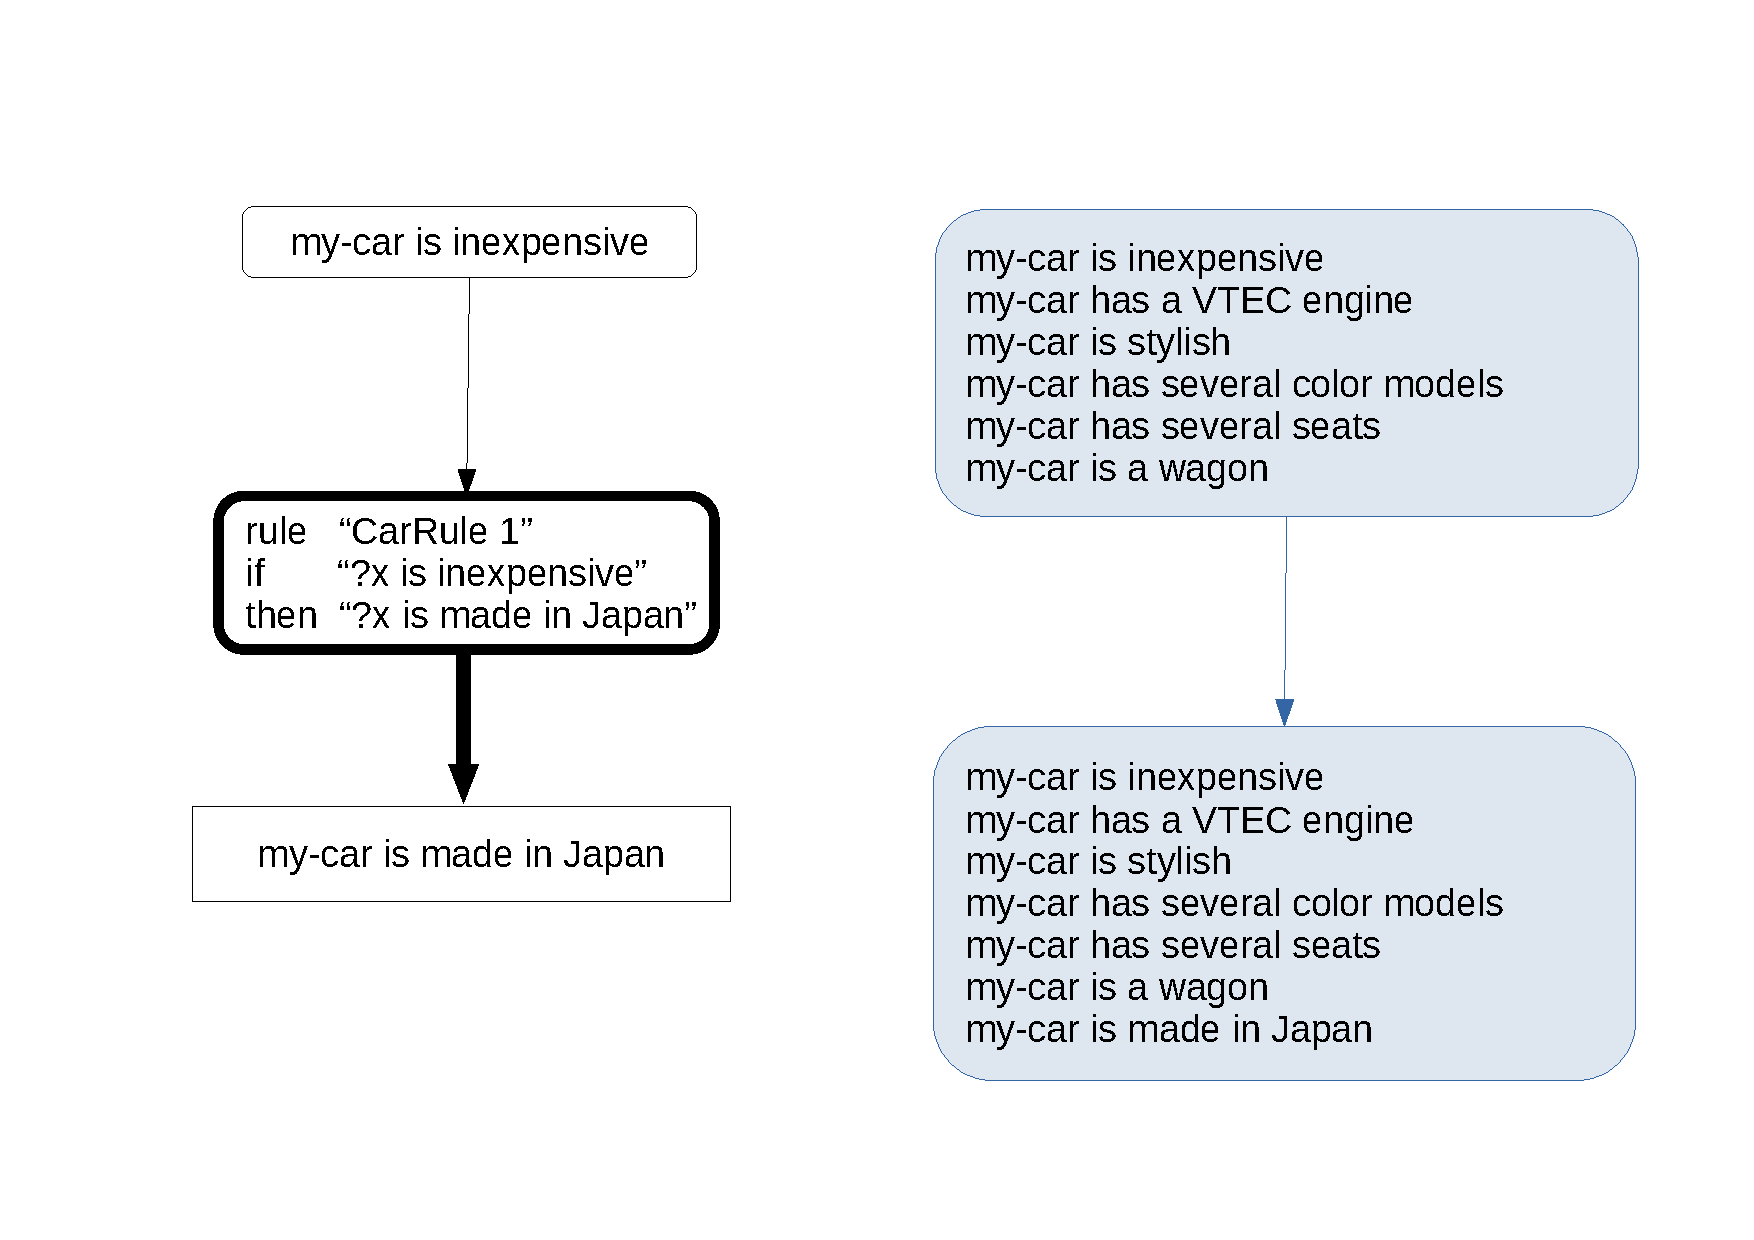
\includegraphics[scale=0.40]{images/forward_chaining_1.pdf}
    \caption{CarRule1の実行とワーキングメモリの変化}
\end{figure}
\newpage
また,上図の右側のワーキングメモリの変化からも読み取れるように,
ルールの実行結果として得られたアサーション"my-car is made in Japan"が実行後のワーキングメモリに追加されている.
このことは,ルールを実行する際の前件にマッチングできる可能性のある知識が増えたことを意味する. \\

続いて,33〜35行目に注目する.
ここでは,ワーキングメモリ内のアサーション"my-car is made in Japan"と"my-car has a VTEC engine"によってCarRule8が実行されている.
したがって,CarRule1の実行結果によって得られた知識を元に推論が駆動されている.
このルールの実行は以下の図の左側のようになる. \\
\begin{figure}[!hbt]
    \centering
    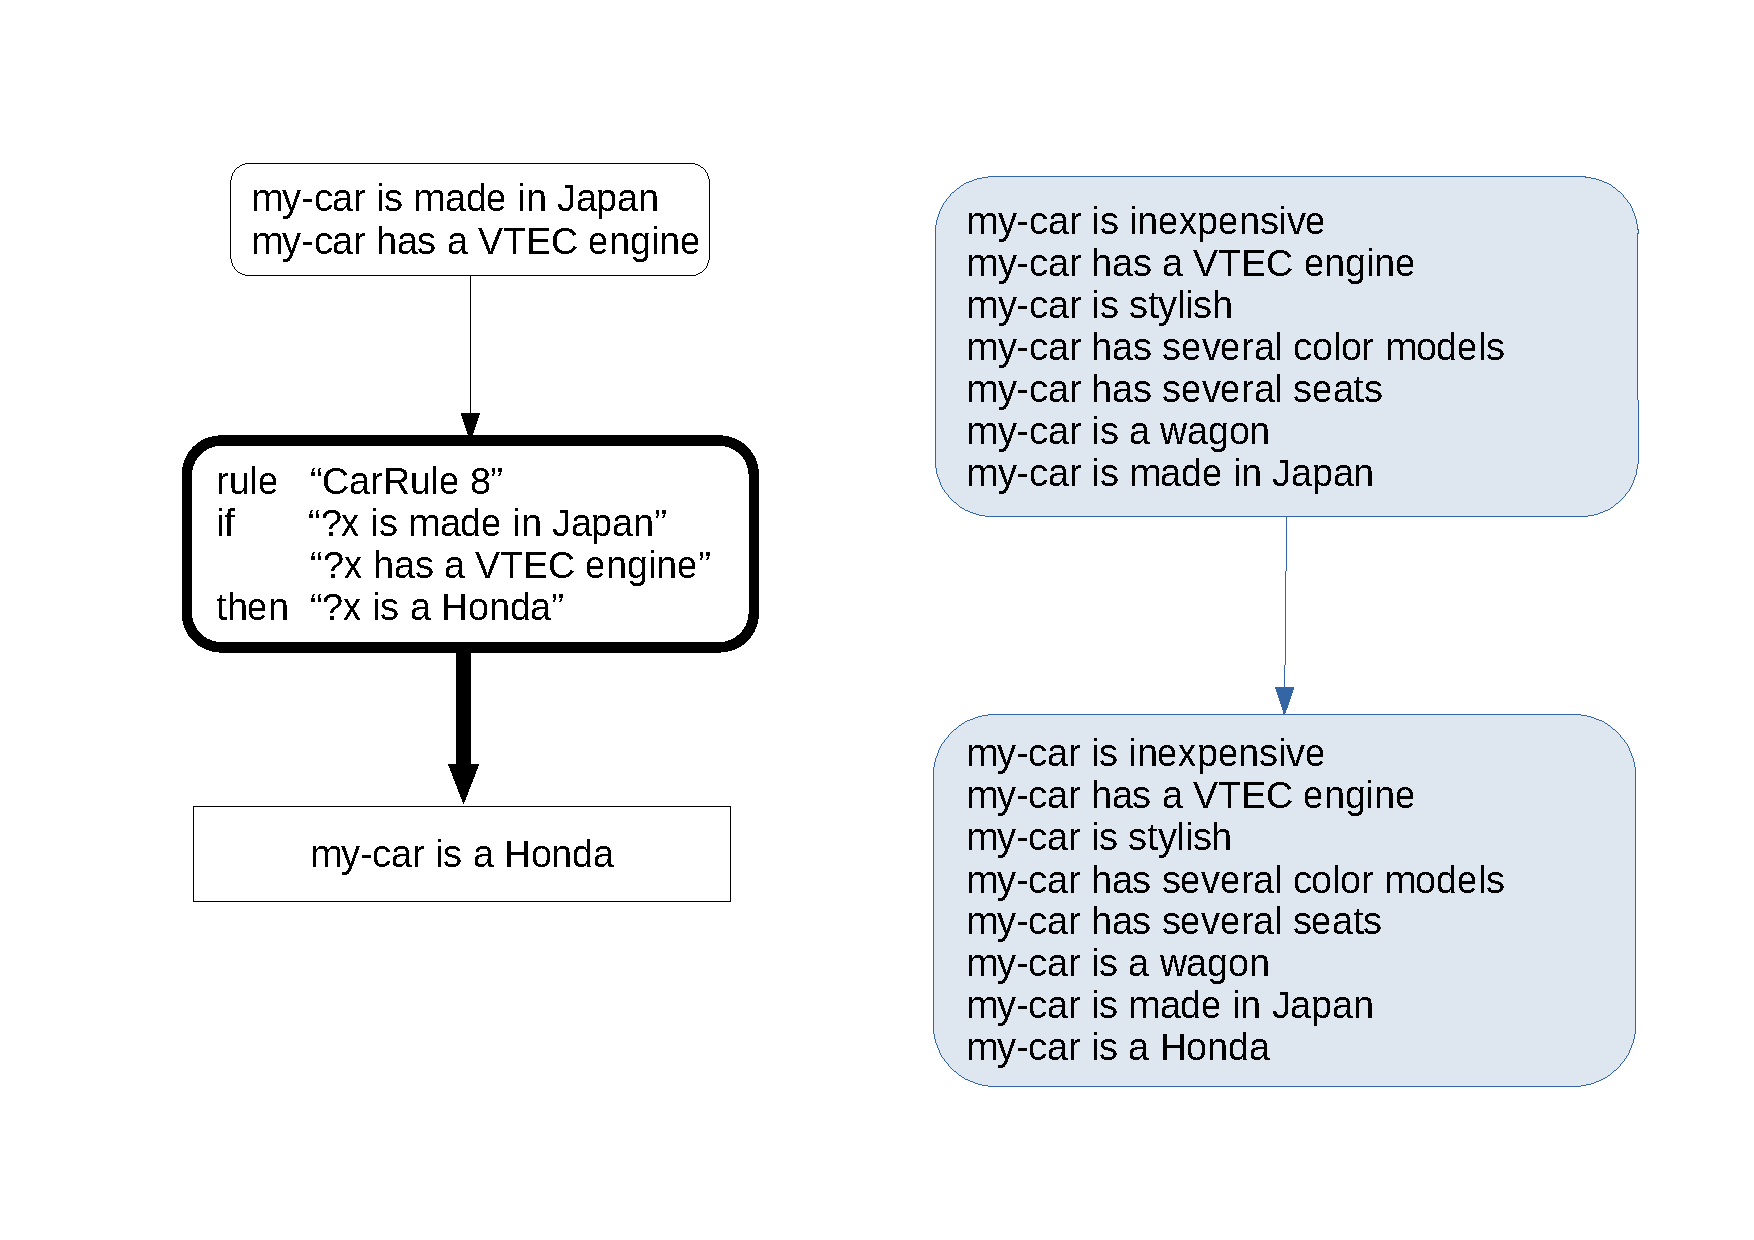
\includegraphics[scale=0.40]{images/forward_chaining_2.pdf}
    \caption{CarRule8の実行とワーキングメモリの変化}
\end{figure}
\newpage
ルールの実行結果として新たなアサーション"my-car is a Honda"がワーキングメモリに追加される. \\

同様に,38〜40行目に着目する.
ここでは,ワーキングメモリ内のアサーション5つを前件にマッチングさせてCarRule11を実行している.
このルールの実行は以下の図の左側のようになる.
\begin{figure}[!hbt]
    \centering
    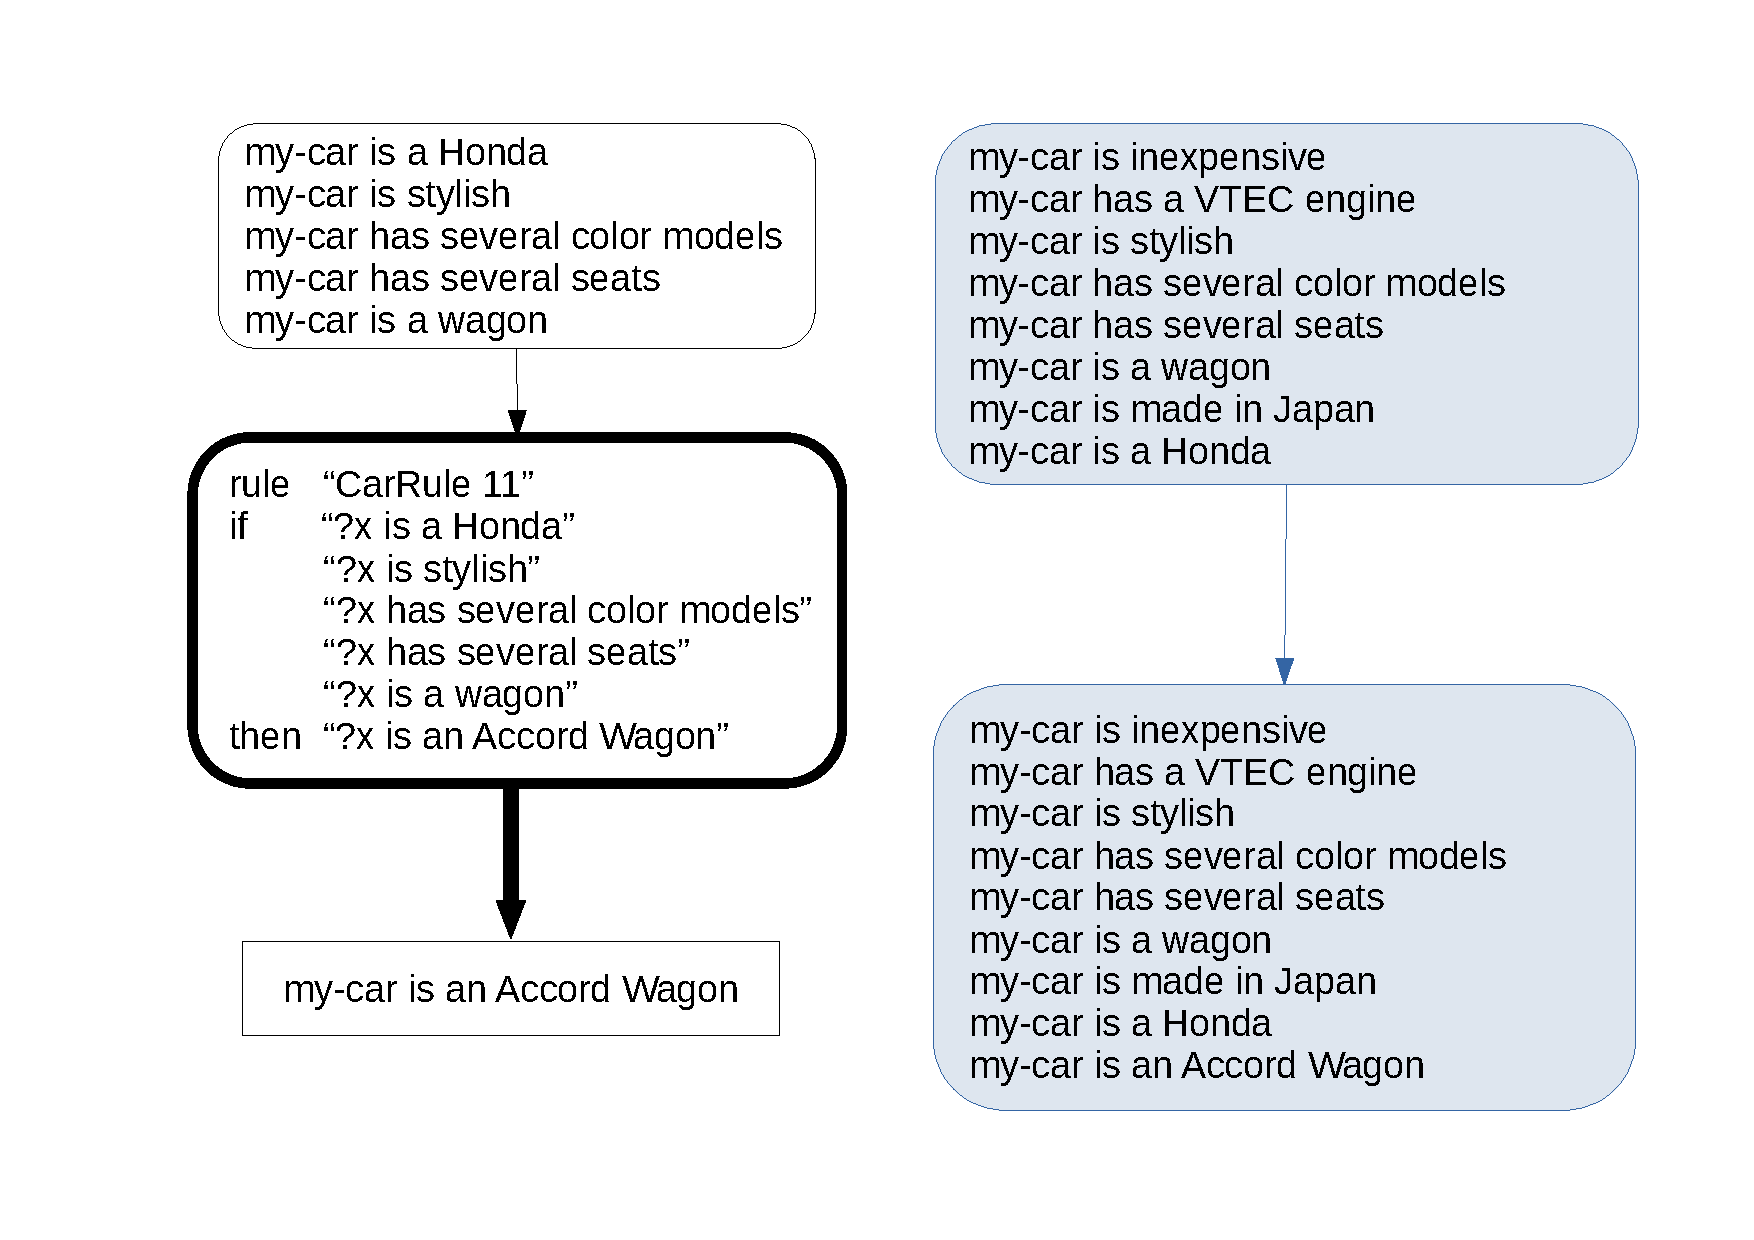
\includegraphics[scale=0.40]{images/forward_chaining_3.pdf}
    \caption{CarRule11の実行とワーキングメモリの変化}
\end{figure}
\newpage
この推論の結果として,新たなアサーション"my-car is an Accord Wagon"が得られた. \\

その後,いかなるルールもマッチングせず,44行目で照合過程が一度終了する.
続く45行目では,現在のワーキングメモリ内部のアサーション集合の確認が行われている. \\
しかし,これで前向き推論のプログラムは終了しない.
46〜60行目にあるように,もう一度照合過程が行われている.
これは,前の照合過程において,あるルールを実行することによって得られた知識を用いて,
そのルールより以前にチェックされたルールが実行される可能性が残されているためである.
この操作は,前向き推論によって網羅的に知識が獲得されていくことを担保する.
ただし,今回の場合は,一周目で全ての知識が獲得されたために,二周目において新たに実行されるルールが存在せず,
62行目にあるように推論が終了している. \\
以上の前向き推論における全ルールの実行過程を示したものを以下に示す.
\begin{figure}[!hbt]
    \centering
    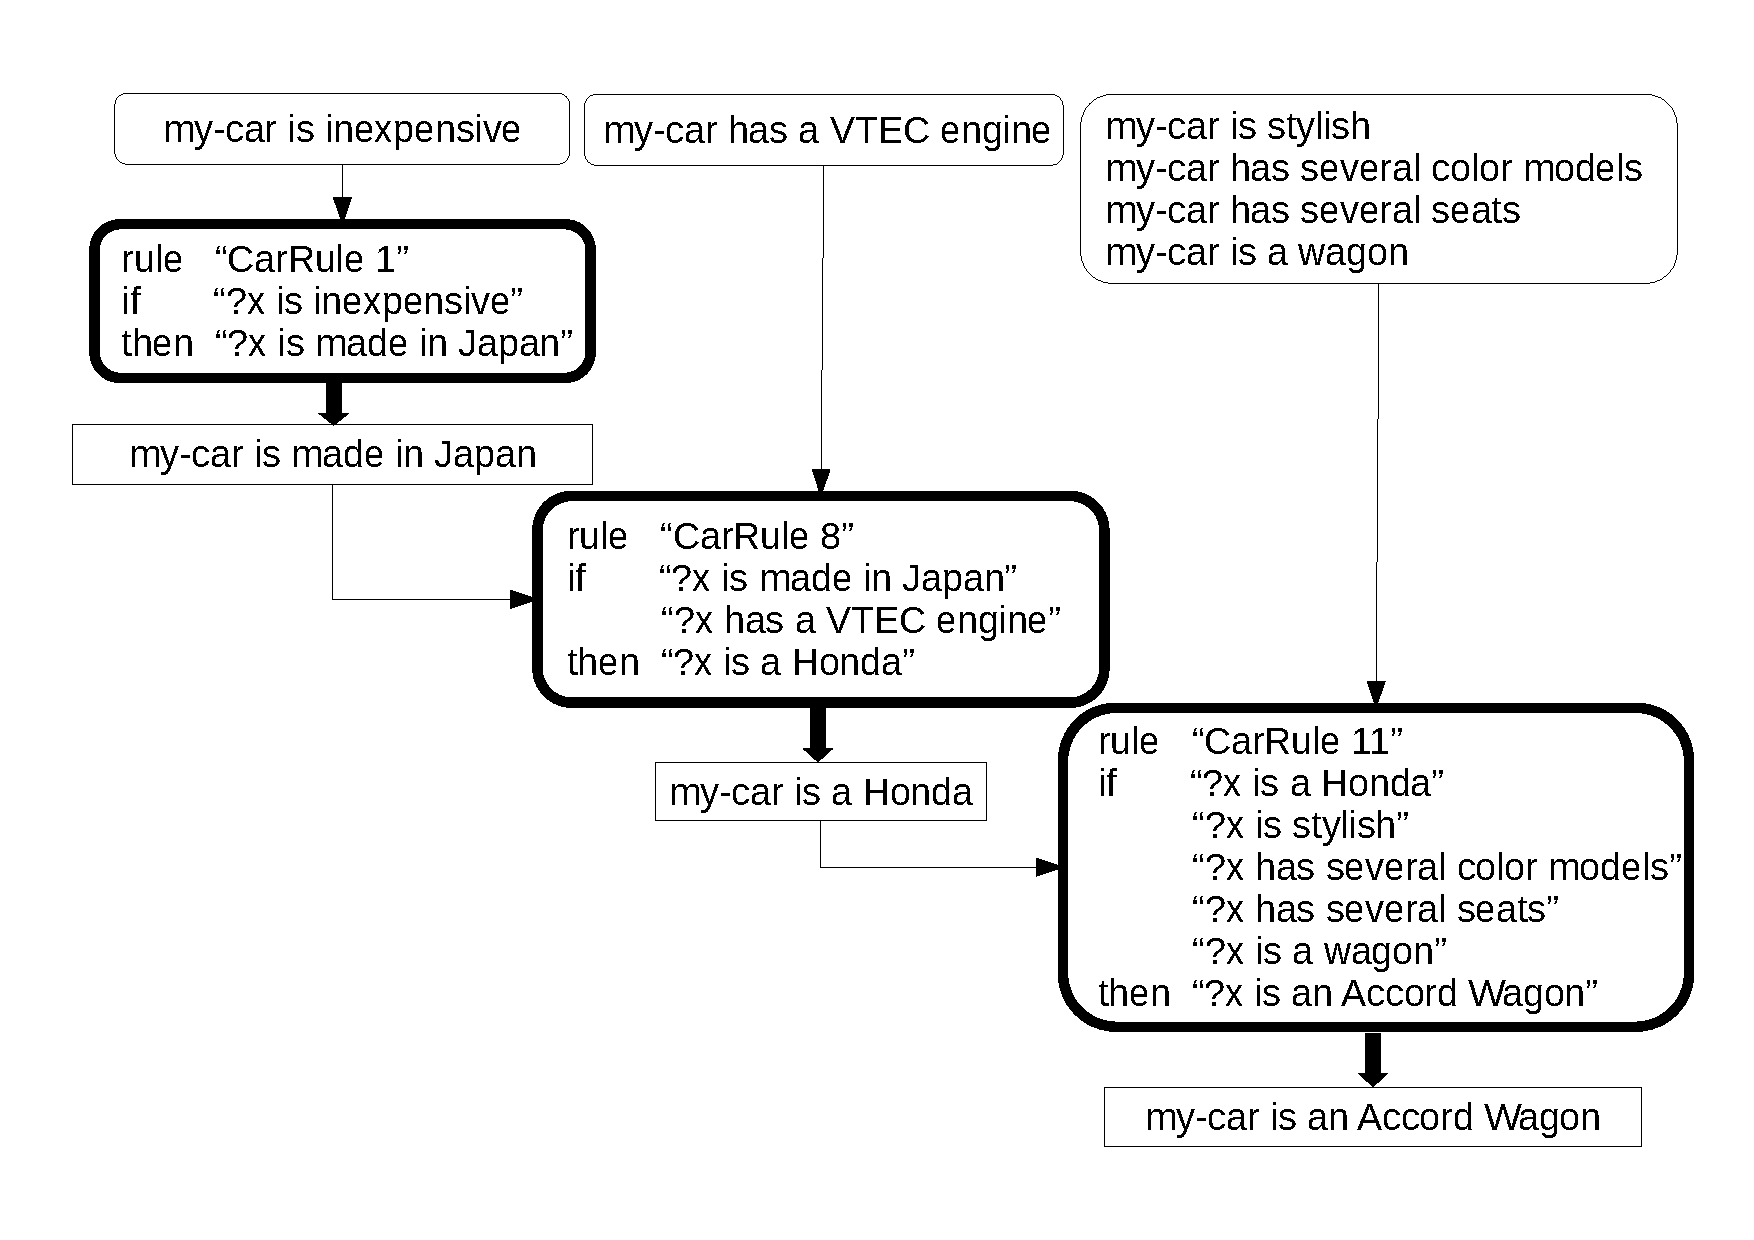
\includegraphics[scale=0.40]{images/forward_chaining_4.pdf}
    \caption{前向き推論の実行}
\end{figure}

\newpage


\subsubsection{後向き推論の実行例について}
以下に,後向き推論の実行結果を示す.
\begin{lstlisting}[caption=後向き推論の実行結果, label=mid]
    ~/Programming2/Work4/BackwordChain
    ●java RuleBaseSystem "?x is an Accord Wagon"                                                                                                                                                                              【 masuda-branch 】
    Hypothesis:[?x is an Accord Wagon]
    Success RULE
    Rule:CarRule11 [?x10 is a Honda, ?x10 is stylish, ?x10 has several color models, ?x10 has several seats, ?x10 is a wagon]->?x10 is an Accord Wagon <=> ?x is an Accord Wagon
    Success RULE
    Rule:CarRule7 [?x17 is made in Japan, ?x17 has Honda's logo]->?x17 is a Honda <=> ?x10 is a Honda
    Success RULE
    Rule:CarRule1 [?x18 is inexpensive]->?x18 is made in Japan <=> ?x17 is made in Japan
    Success WM
    his-car is inexpensive <=> ?x18 is inexpensive
    tmpPoint: 12
    Success:?x17 is made in Japan
    tmpPoint: -1
    Success RULE
    Rule:CarRule8 [?x37 is made in Japan, ?x37 has a VTEC engine]->?x37 is a Honda <=> ?x10 is a Honda
    Success RULE
    Rule:CarRule1 [?x38 is inexpensive]->?x38 is made in Japan <=> ?x37 is made in Japan
    Success WM
    his-car is inexpensive <=> ?x38 is inexpensive
    tmpPoint: 12
    Success:?x37 is made in Japan
    Success WM
    his-car has a VTEC engine <=> ?x37 has a VTEC engine
    tmpPoint: 19
    Success:?x10 is a Honda
    Success WM
    his-car is stylish <=> ?x10 is stylish
    tmpPoint: 3
    Success:?x10 is stylish
    Success WM
    his-car has several color models <=> ?x10 has several color models
    tmpPoint: 4
    Success:?x10 has several color models
    Success WM
    his-car has several seats <=> ?x10 has several seats
    tmpPoint: 5
    Success:?x10 has several seats
    Success WM
    his-car is a wagon <=> ?x10 is a wagon
    Yes
    {?x38=his-car, ?x37=his-car, ?x10=his-car, ?x=his-car}
    binding: {?x38=his-car, ?x37=his-car, ?x10=his-car, ?x=his-car}
    tmp: ?x, result:  his-car
    Query: ?x is an Accord Wagon
    Answer:his-car is an Accord Wagon
\end{lstlisting}
まず,2行目では,コマンドとして java RuleBaseSystem "?x is an Accord Wagon" を実行しており,条件を満たすような?xを問う形式になっている.
この後向き推論では,この?xを変数束縛として具体化することによって得ることを目的とする.
ゆえに,実行例の3行目では,大元の仮説として"?x is an Accord Wagon"が設定されている. \\
後向き推論では,仮説とルールの後件をマッチングさせることによって次の仮説を導き出し,仮説とワーキングメモリ内のアサーションのマッチングを行うことで変数束縛を行う.
したがって,この2点に注目して実行例の解説を行うものとする.
なお,バックトラック等の複雑な処理の解説も行うため,説明量がやや多くなることを断っておく. \\

実行例の4・5行目では,CarRule11の後件と仮説のマッチングが成功している.
すなわち,"?x10 is an Accord Wagon"と"?x is an Accord Wagon"の間でマッチングが成功し,?x=?x10として束縛される.
以下の図5に,このマッチングの様子を示す.
\begin{figure}[!hbt]
    \centering
    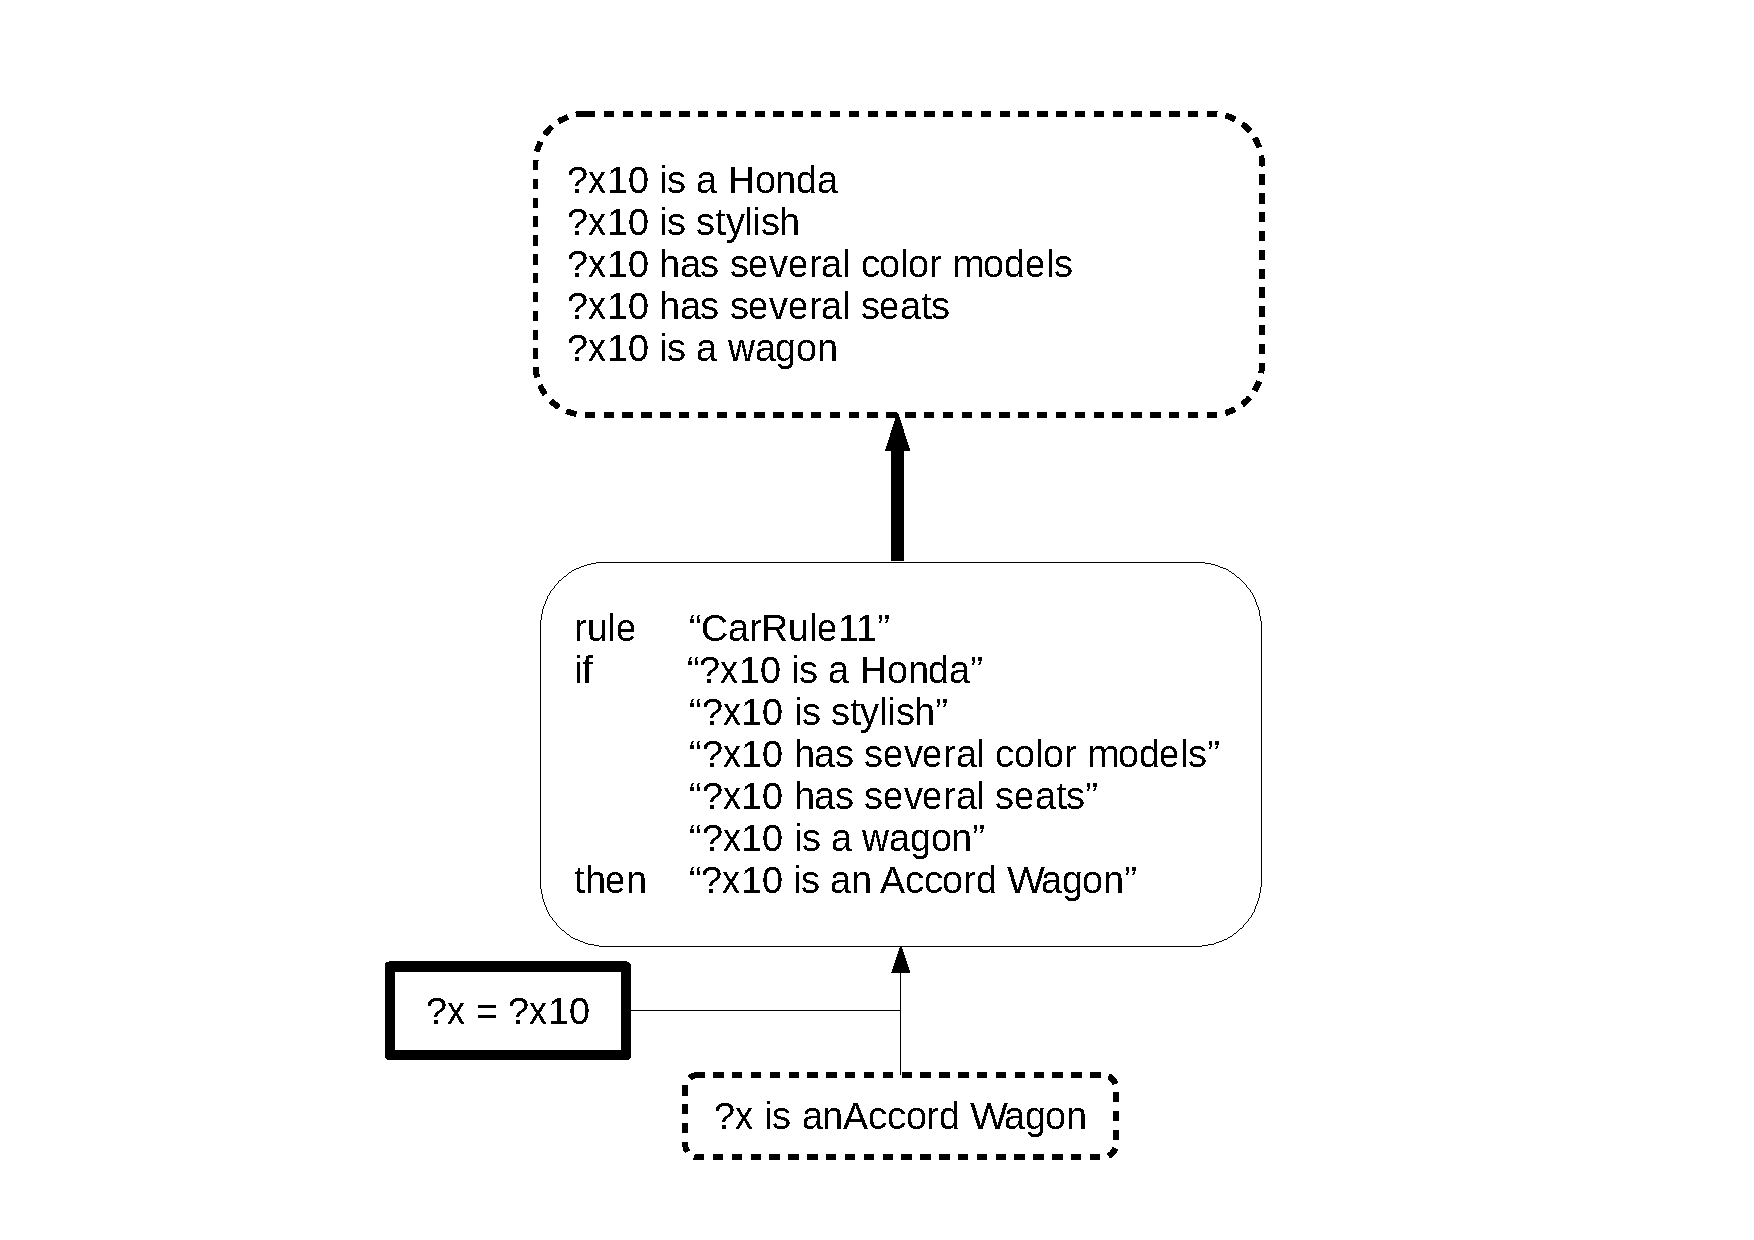
\includegraphics[scale=0.30]{images/backward_chaining_1.pdf}
    \caption{CarRule11の後件と仮説のマッチング}
\end{figure}
その結果として,CarRule11の前件
[?x10 is a Honda, ?x10 is stylish, ?x10 has severalcolor models, ?x10 has several seats, ?x10 is a wagon]
が新たな仮定として導出される.
これらの仮定が真となれば,元の仮定も真となる. \\

次に,実行例6・7行目においてCarRule7の後件と新たに導出された仮説の一つ"?x10 is a Honda"のマッチングが成功している.
詳細については以下の図6に示す.
\begin{figure}[!hbt]
    \centering
    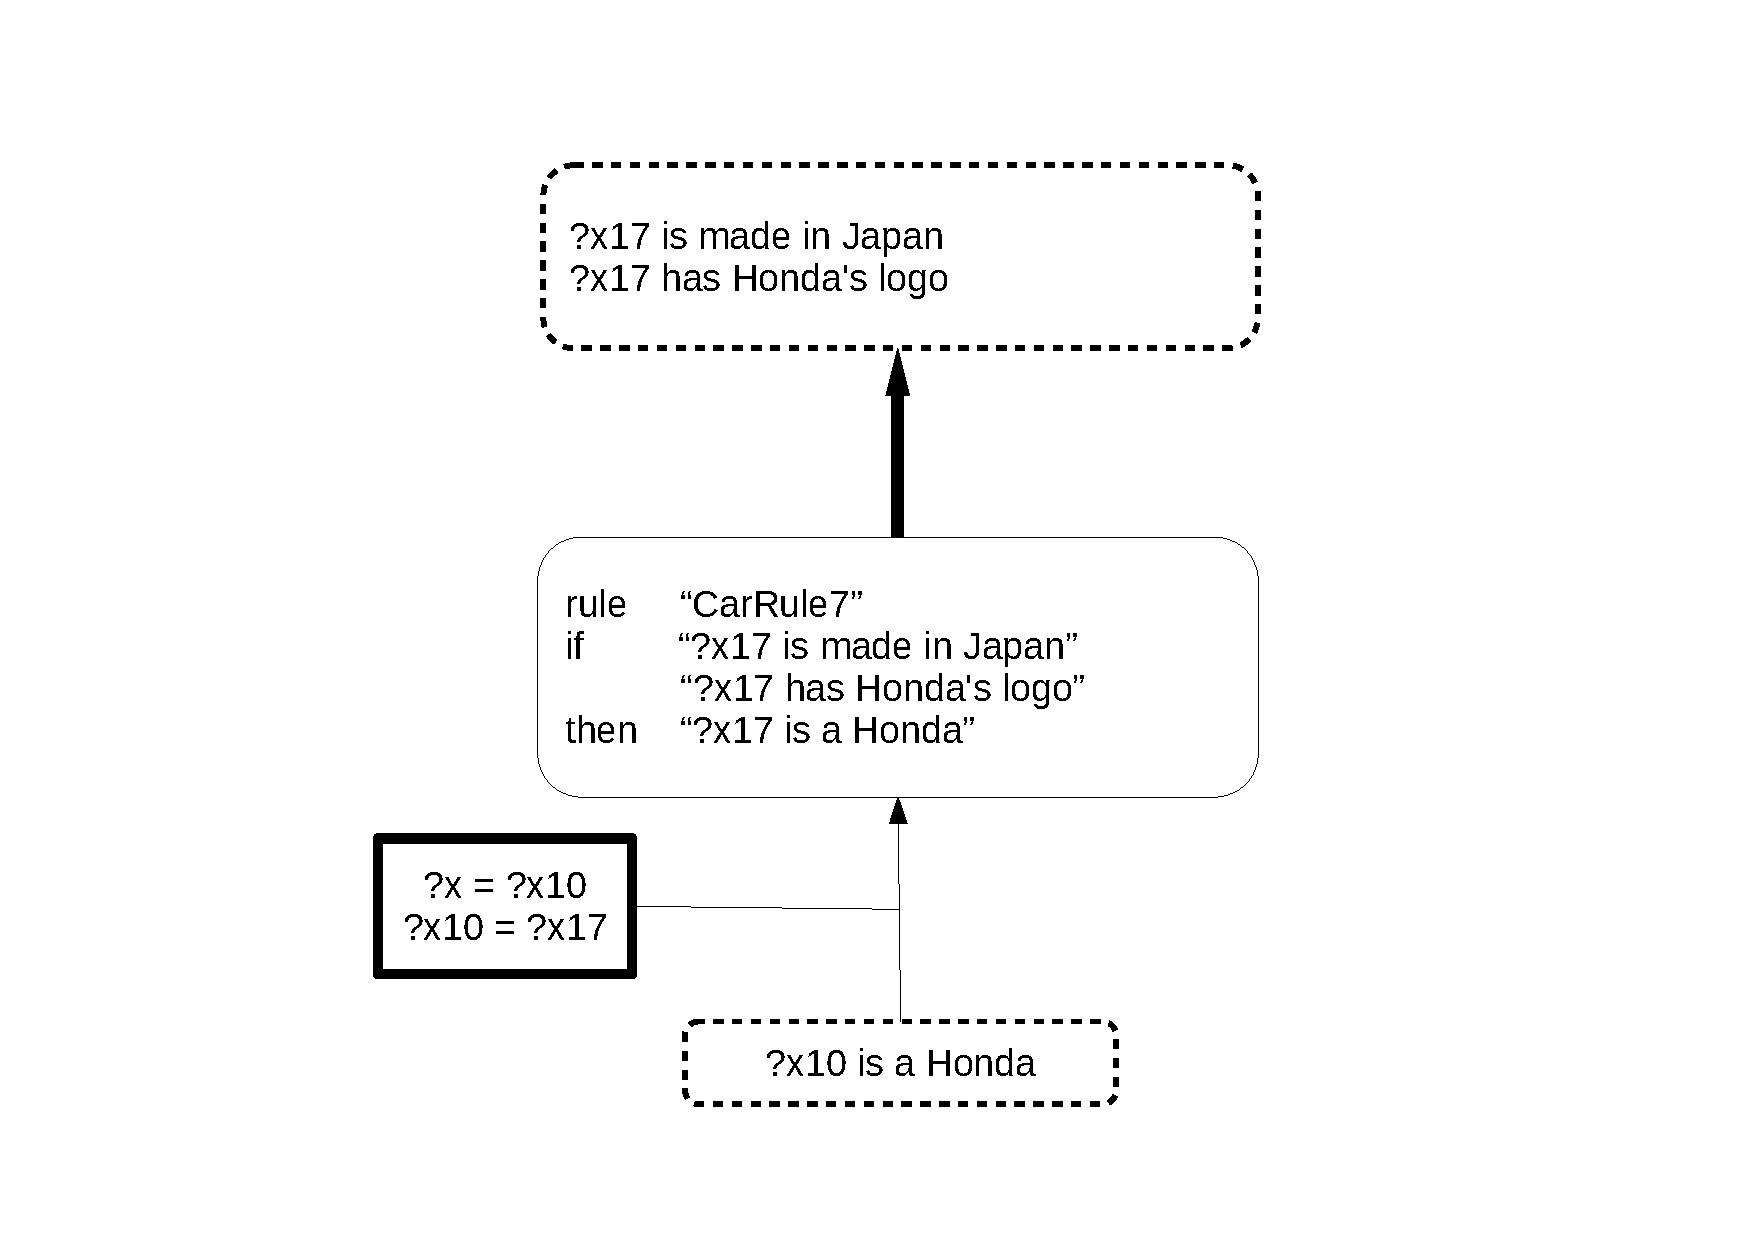
\includegraphics[scale=0.30]{images/backward_chaining_2.pdf}
    \caption{CarRule7の後件と仮説のマッチング}
\end{figure}
結果として,仮説"?x10 is a Honda"は[?x17 is made in Japan, ?x17 has Honda's logo]に置き換わった. \\

同様にして,実行例8・9行目においても以下の図7のように仮説が置き換わる.
\begin{figure}[!hbt]
    \centering
    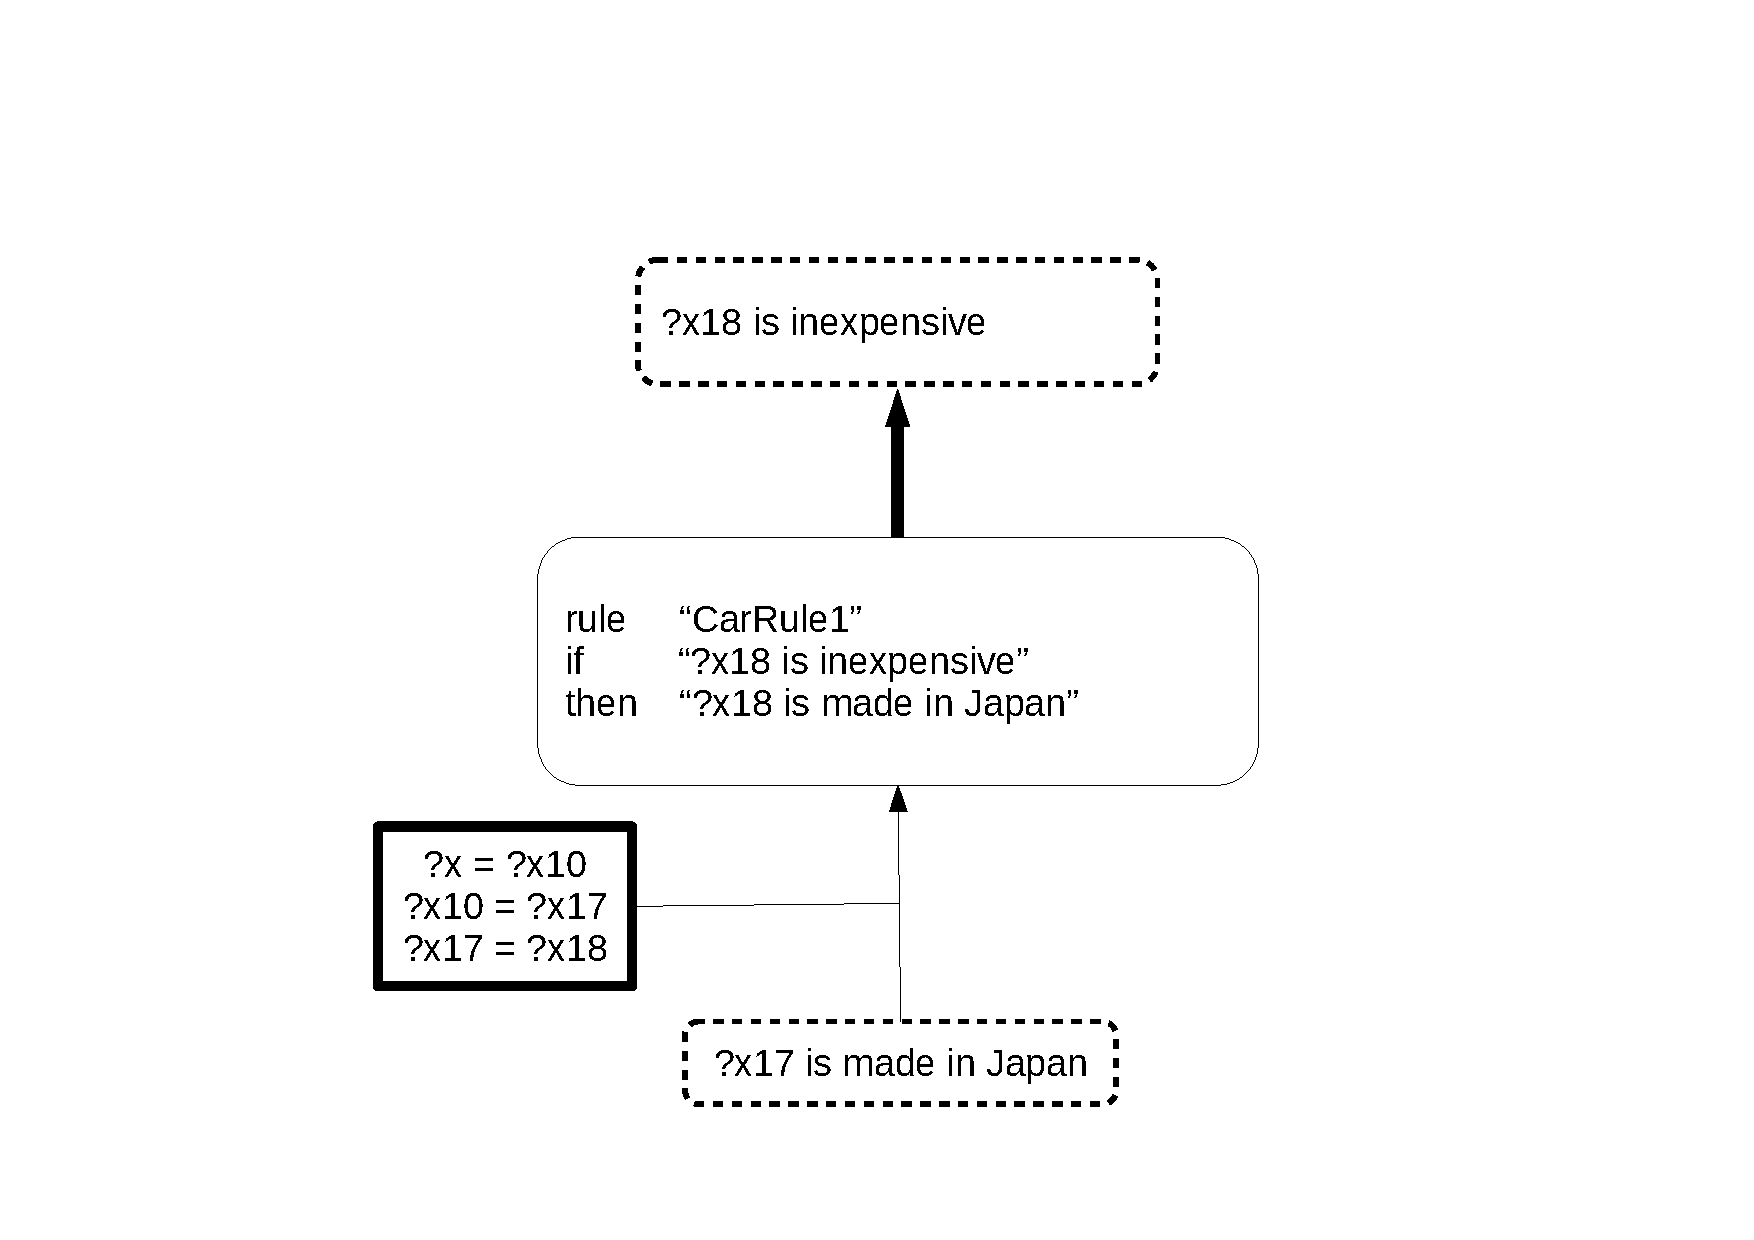
\includegraphics[scale=0.30]{images/backward_chaining_3.pdf}
    \caption{CarRule1の後件と仮説のマッチング}
\end{figure}

次に,10〜12行目において,先ほどのマッチングの結果によって得られた仮説の具体化が行われている.
すなわち,"?x18 is inexpensive"とワーキングメモリ内のアサーション"his-car is inexpensive"
が一致することによって,変数?x18=?x17=?x10=?x=his-carとして具体化が得られる.
以下の図8に具体化の様子を示す.
\begin{figure}[!hbt]
    \centering
    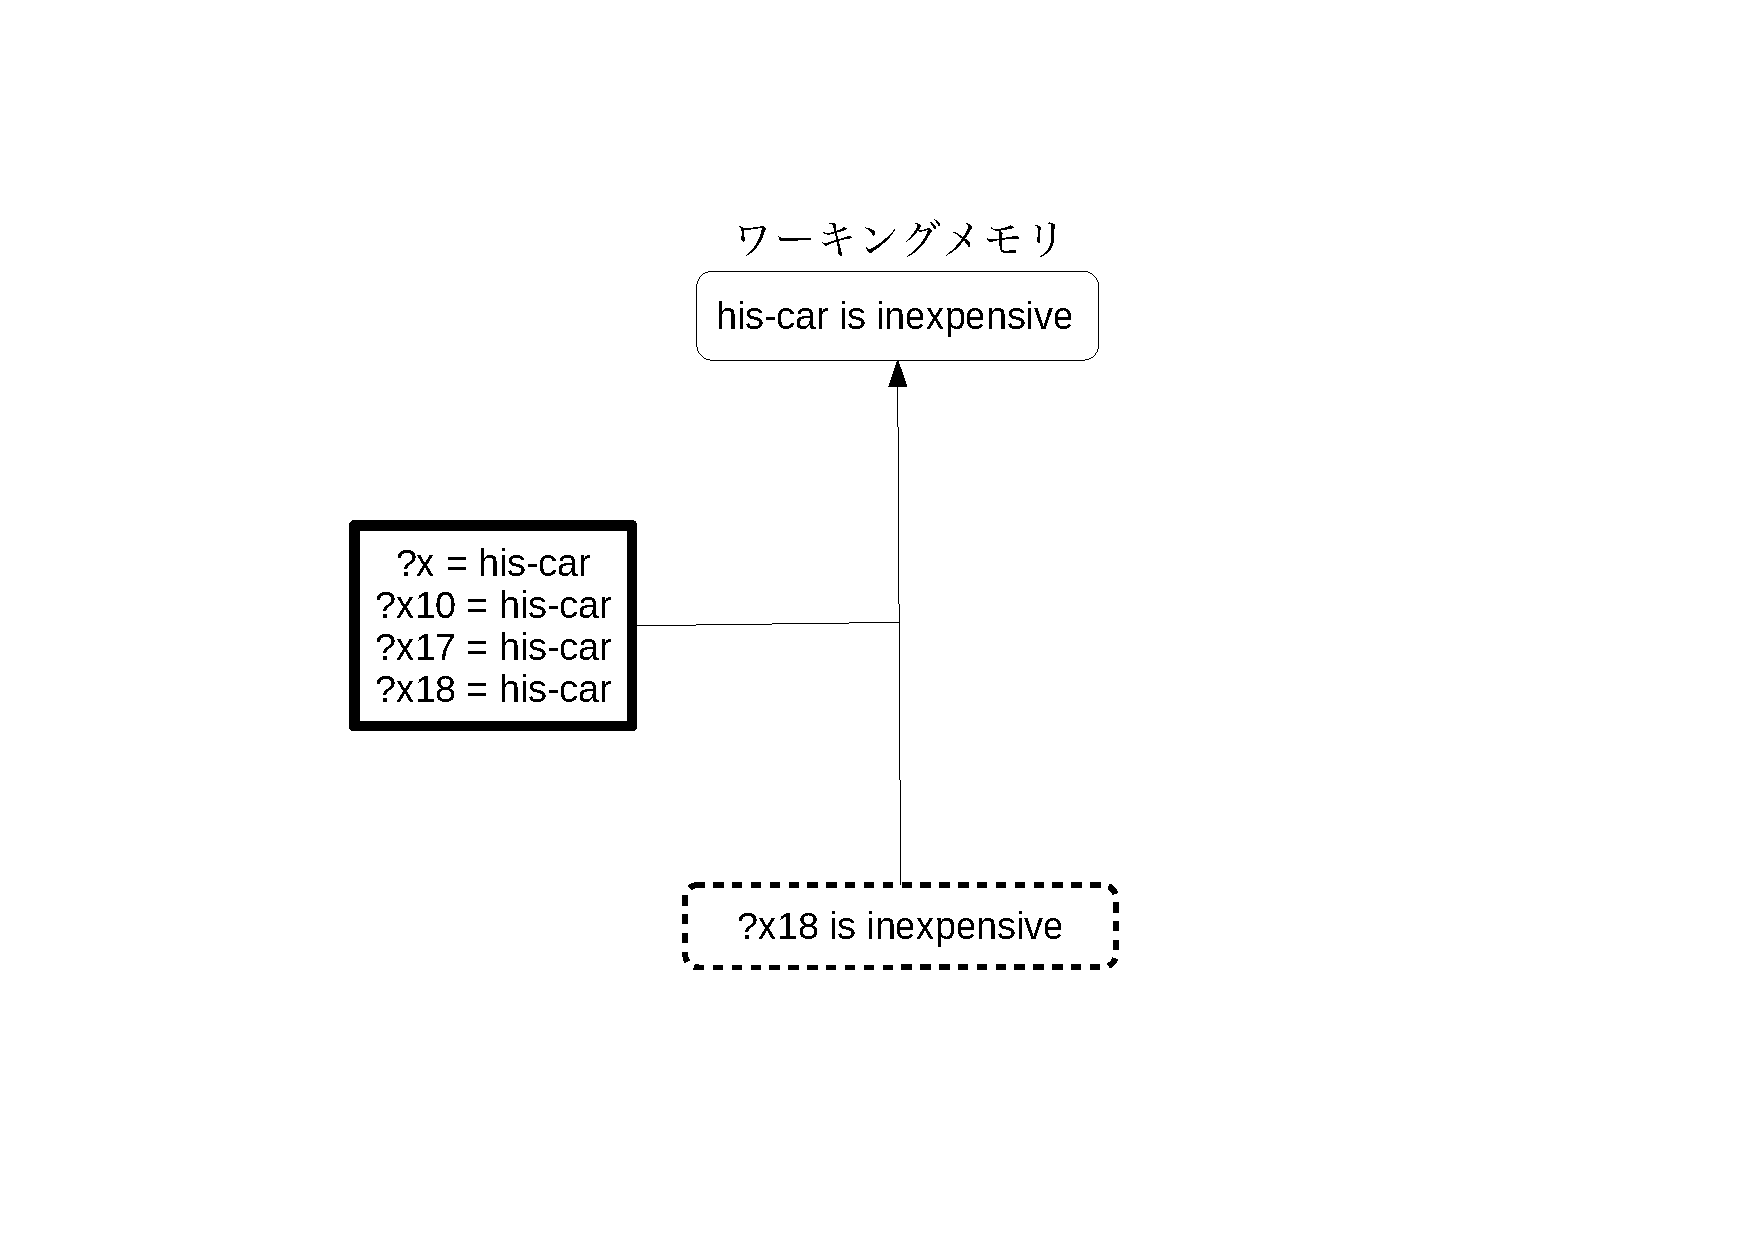
\includegraphics[scale=0.30]{images/backward_chaining_4.pdf}
    \caption{"?x18 is inexpensive"と"his-car is inexpensive"による具体化}
\end{figure}
これにより,他の仮説についても?x18=?x17=?x10=?x=his-carとして具体化されたものが,
ワーキングメモリ内のアサーション集合に存在すれば元の仮説が真となる.
13行目では,この具体化を受けて仮説"?x17 is made in Japan"が成功したことが示されている. \\

\newpage

しかし,ここで問題が発生する.
先ほど,?x18=?x17=?x10=?x=his-carによる具体化が得られたが,
CarRule7により導かれた仮説の一つである"?x17 has Honda's logo"
について,?x17=his-carとした時のアサーション"his-car has Honda's logo"が存在しないのである.
したがって,仮説"?x17 has Honda's logo"は偽となり,tmpPointは-1を返すこととなる.
以下の図9に仮説のマッチングの失敗を図示する.
\begin{figure}[!hbt]
    \centering
    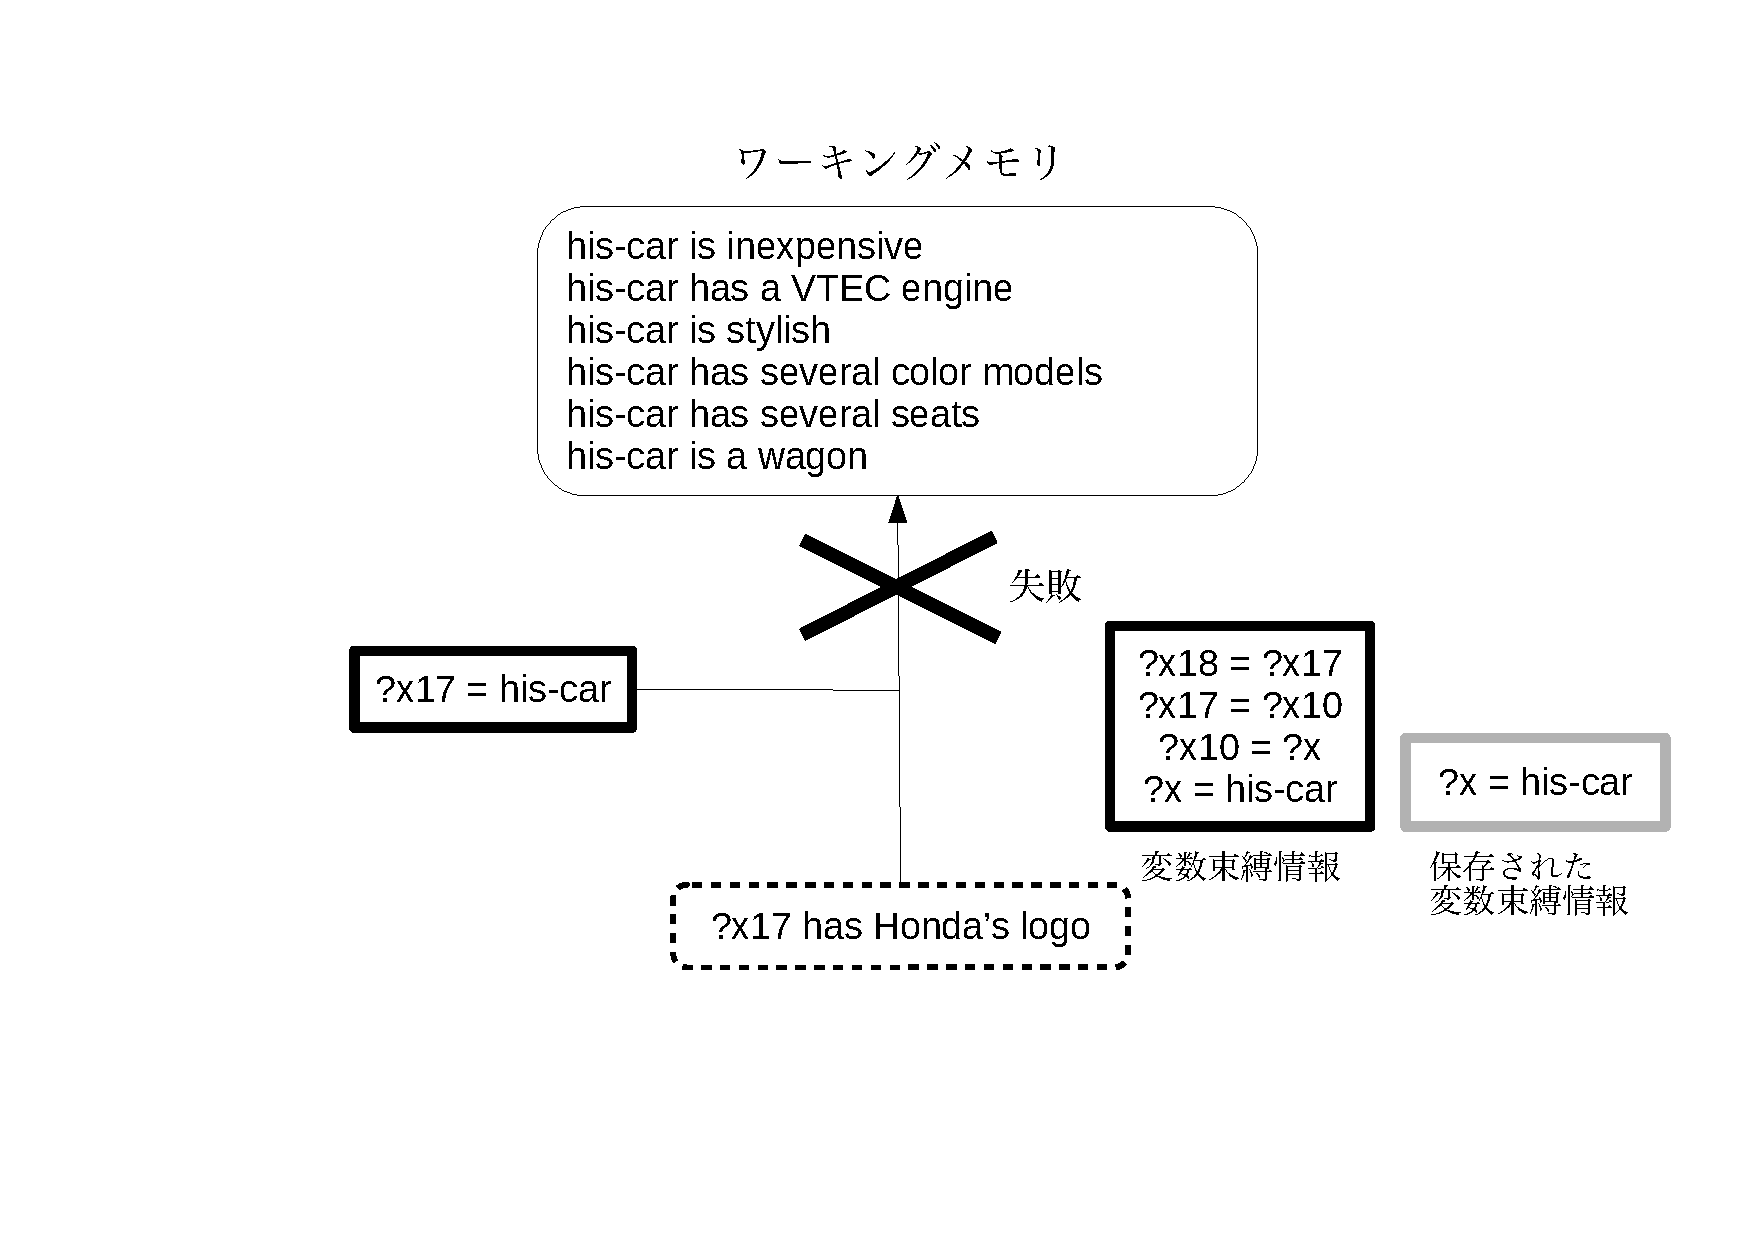
\includegraphics[scale=0.30]{images/backward_chaining_5.pdf}
    \caption{仮説"his-car has Honda's logo"の失敗}
\end{figure}
この図から,ワーキングメモリ内に該当アサーション"his-car has Honda's logo"が存在しないことが確認できる.
これにより,CarRule7により,仮説"?x10 is Honda"を導くことが不可能であることが示された. \\

仮説のチェックの失敗により,一つ前の推論ステップに戻ってCarRule7の代わりとなる新たなルールを探す必要が生じる.
この一連の処理のことをバックトラックと呼び,先ほどユニフィケーションされた変数束縛は元に戻される.
すなわち,変数束縛情報は?x10=?xの状態に再び戻る.
以下の図10,バックトラックの実行を示す.
\begin{figure}[!hbt]
    \centering
    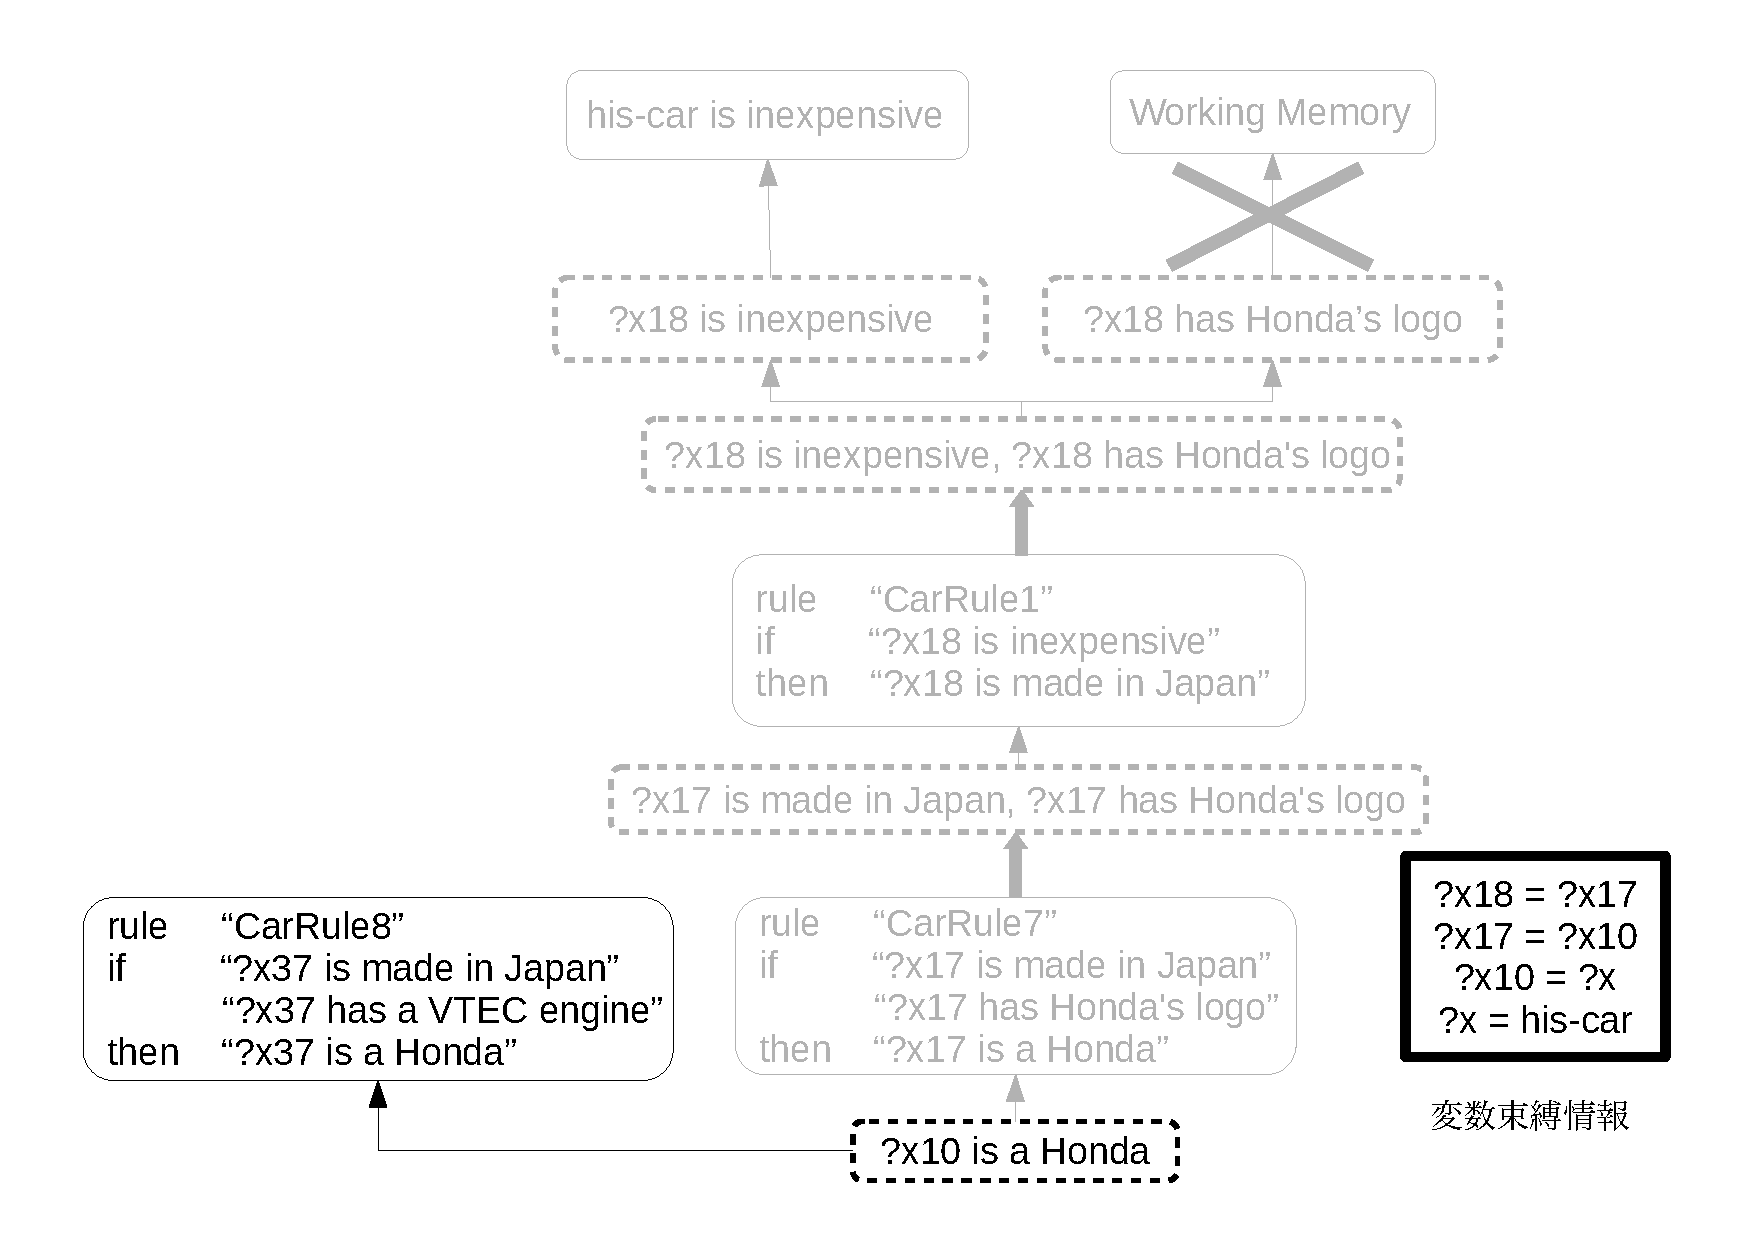
\includegraphics[scale=0.40]{images/backward_chaining_6.pdf}
    \caption{バックトラックの実行}
\end{figure}
バックトラックの実行によって,再び仮説"?x10 is a Honda"を真にするような仮説を導出するルールを探すこととなった. \\

\newpage

そして,15・16行目において,CarRule8の後件と"?x10 is a Honda"のパターンマッチングが成功する.
これについても詳細は以下の図11に示すものとする.
\begin{figure}[!hbt]
    \centering
    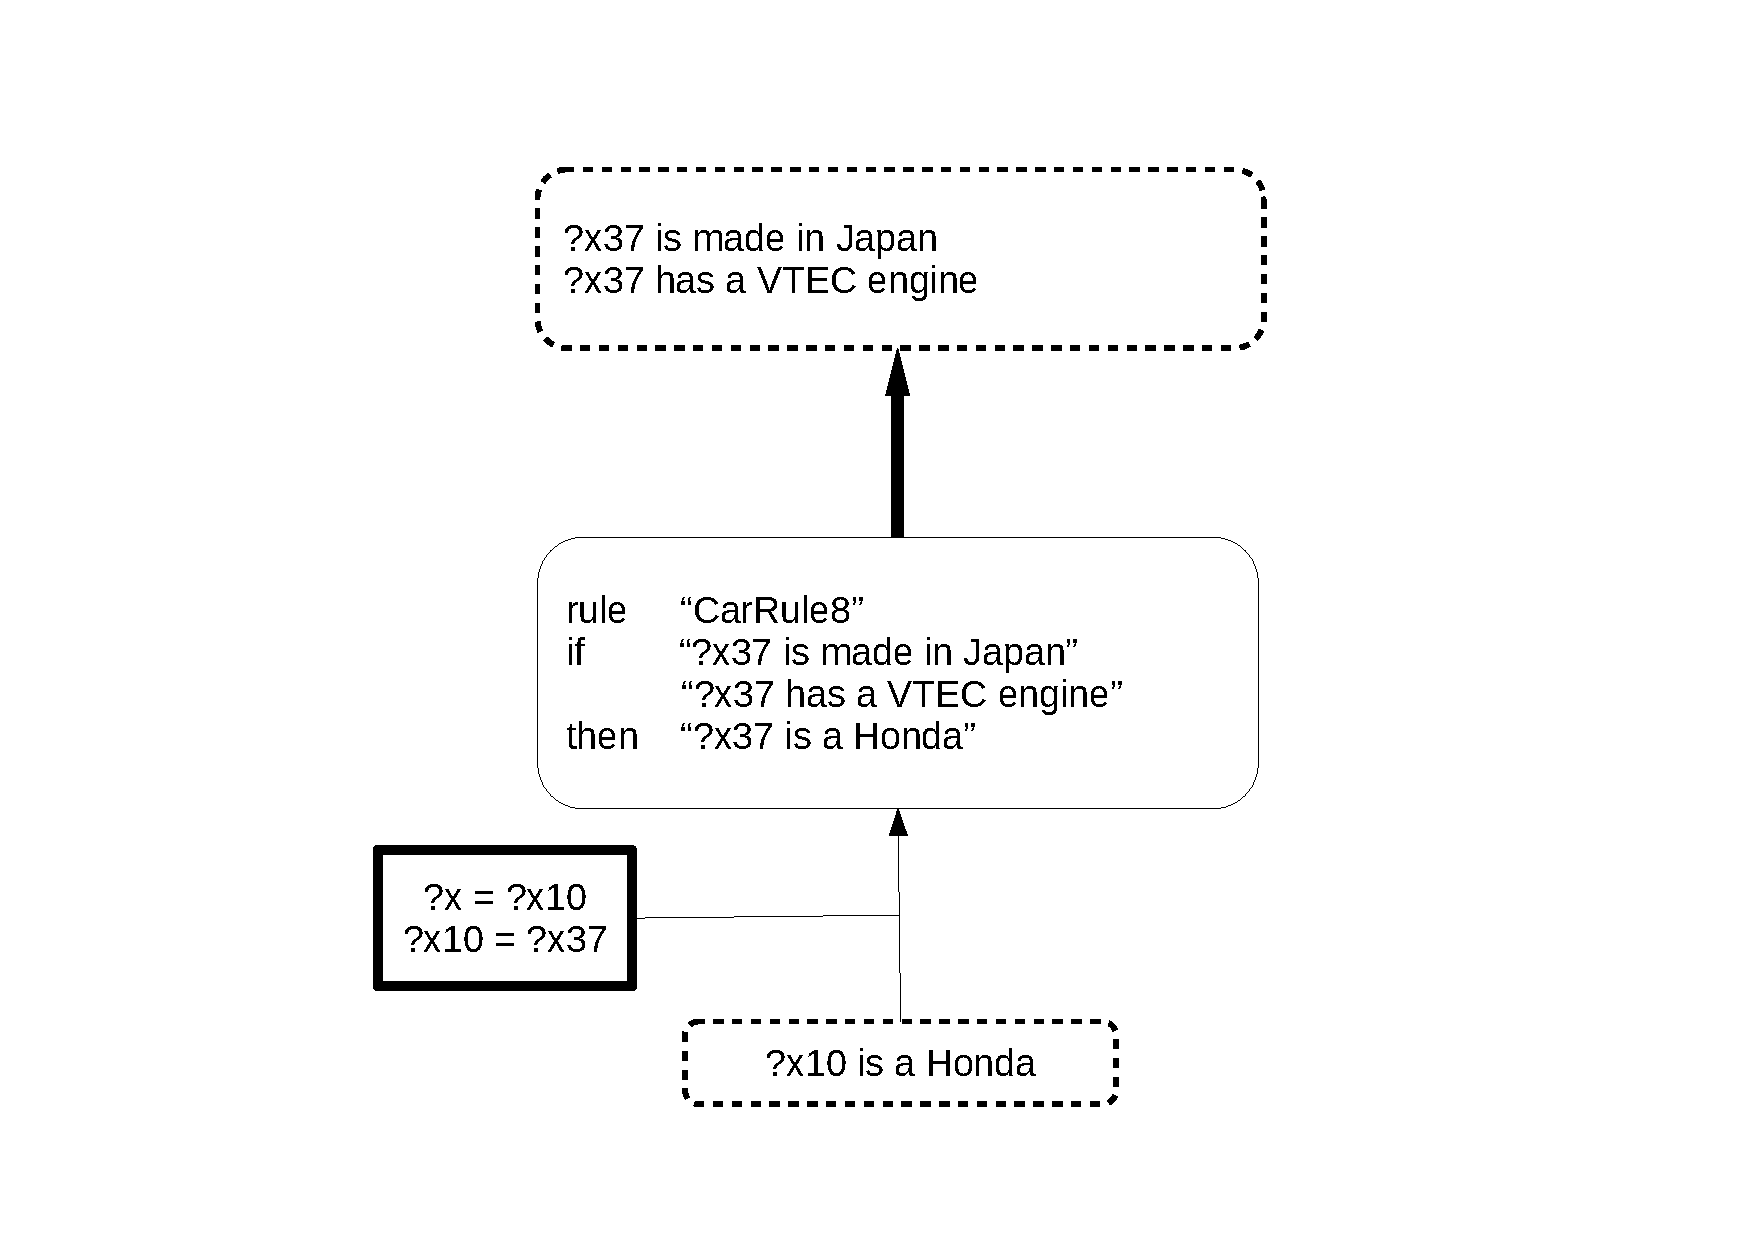
\includegraphics[scale=0.30]{images/backward_chaining_7.pdf}
    \caption{CarRule8の後件と仮説のマッチング}
\end{figure}

同様に,17・18行目でもCarRule1の後件と"?x37 is made in Japan"のマッチングを示す.
図12を参照する.
\begin{figure}[!hbt]
    \centering
    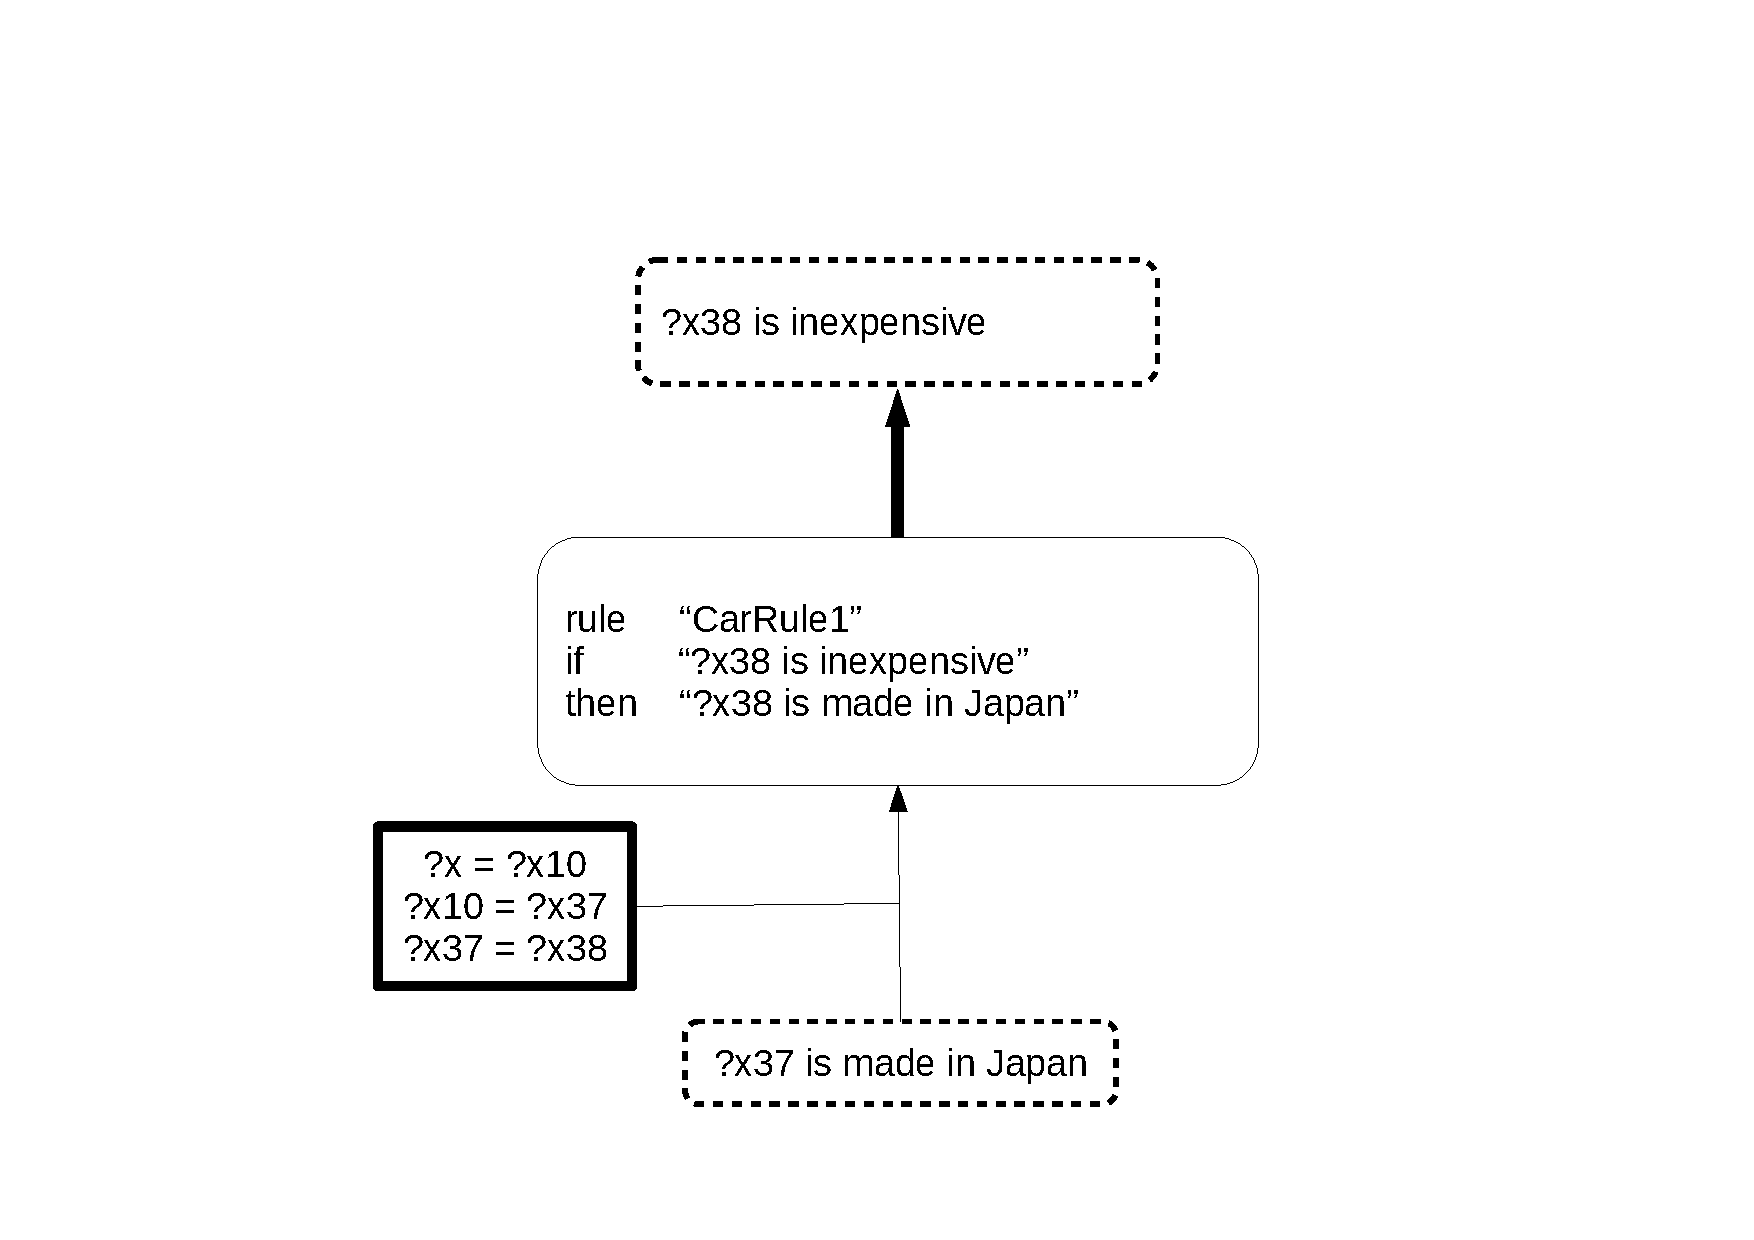
\includegraphics[scale=0.30]{images/backward_chaining_8.pdf}
    \caption{CarRule1の後件と仮説のマッチング}
\end{figure}

\newpage

実行例19・20行目でようやく"his-car is inexpensive"と"?x38 is inexpensive"によって具体化が得られる.
すなわち,?x38=?x37=?x10=?x=his-carが得られる.
\begin{figure}[!hbt]
    \centering
    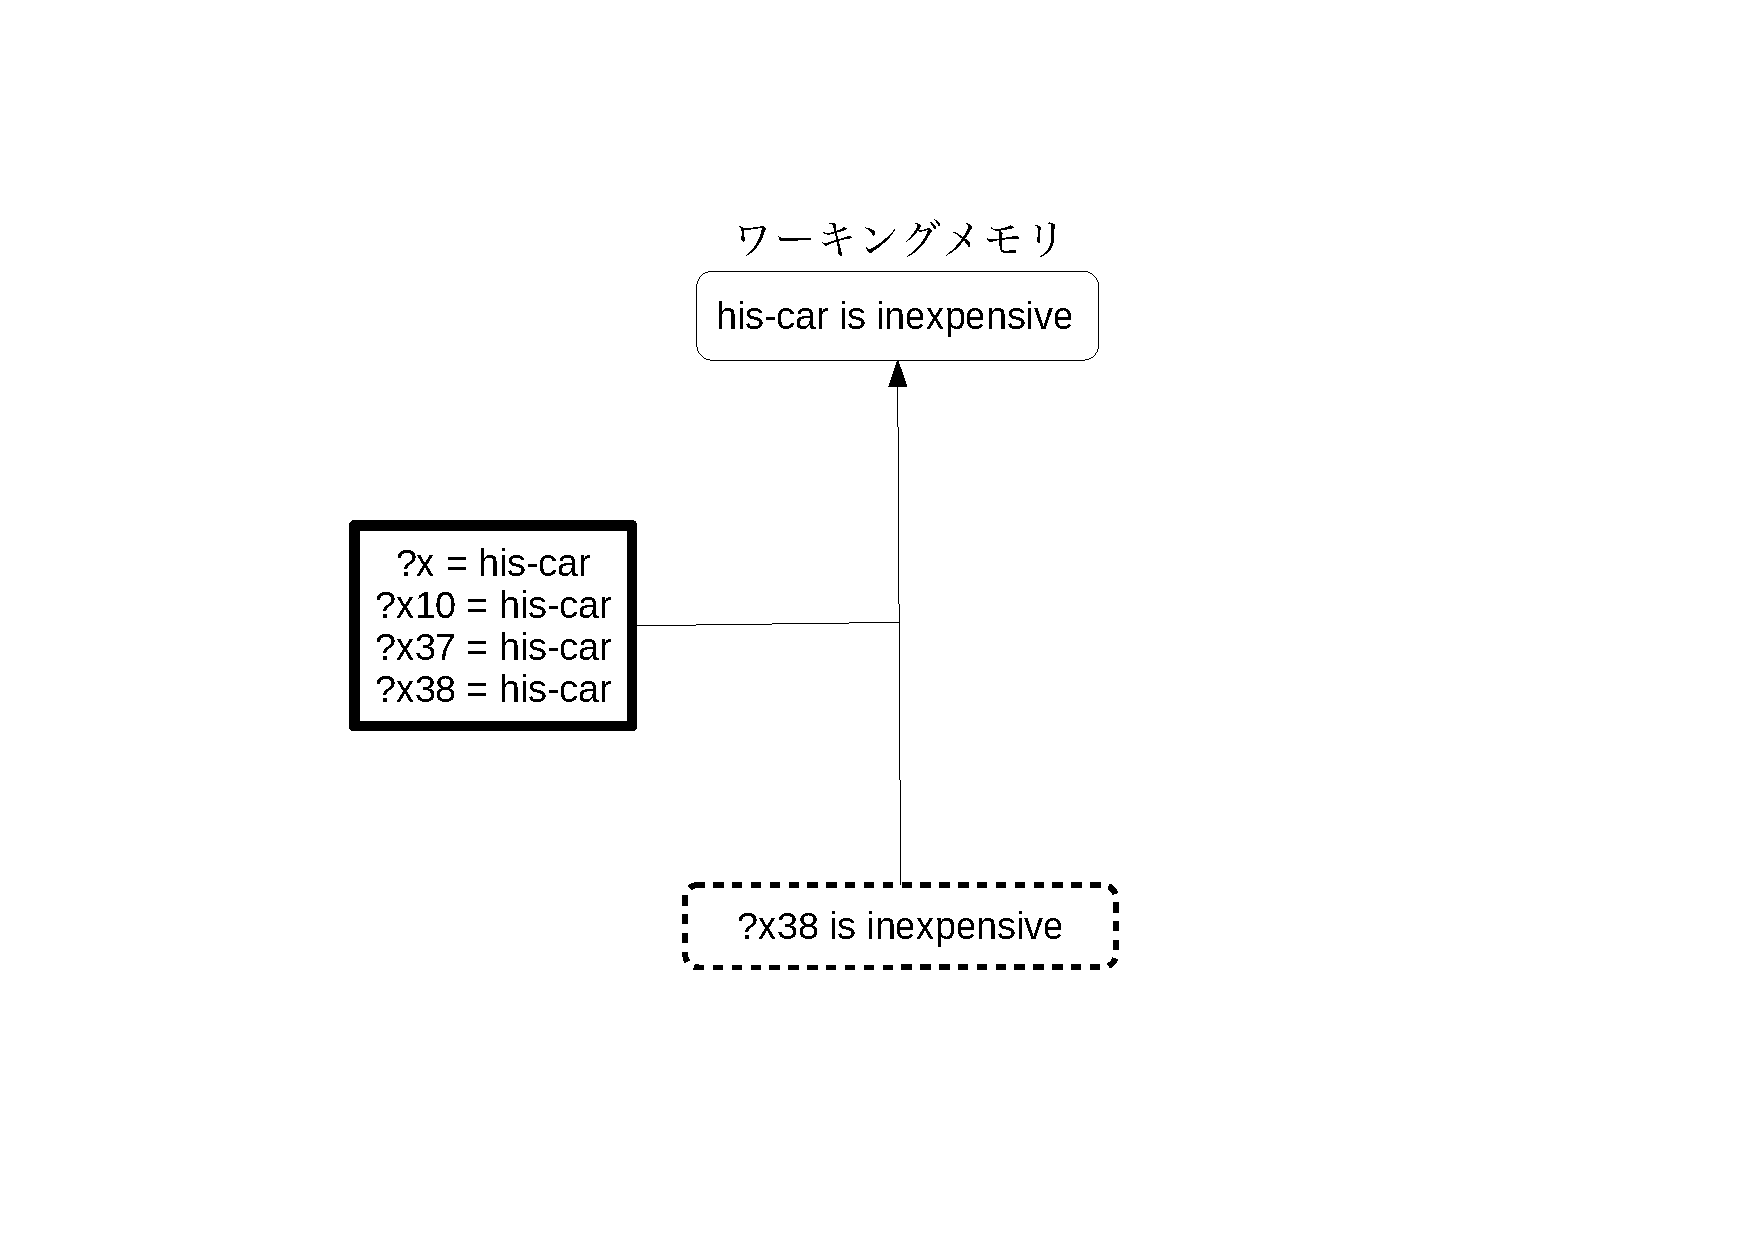
\includegraphics[scale=0.30]{images/backward_chaining_9.pdf}
    \caption{"his-car is inexpensive"と"?x38 is inexpensive"によるユニフィケーション}
\end{figure}

先ほどのユニフィケーションの結果を受けて,?x37=his-carとなるので,仮説"?x37 has a VTEC engine"が真となるためには,
ワーキングメモリ内のアサーション集合に"his-car has a VTEC engine"が含まれれば良い.
ワーキングメモリ内を確認すると,"his-car has a VTEC engine"は存在するので,この仮説は真である.
以下,図14に仮説のチェックの過程を示す.
\begin{figure}[!hbt]
    \centering
    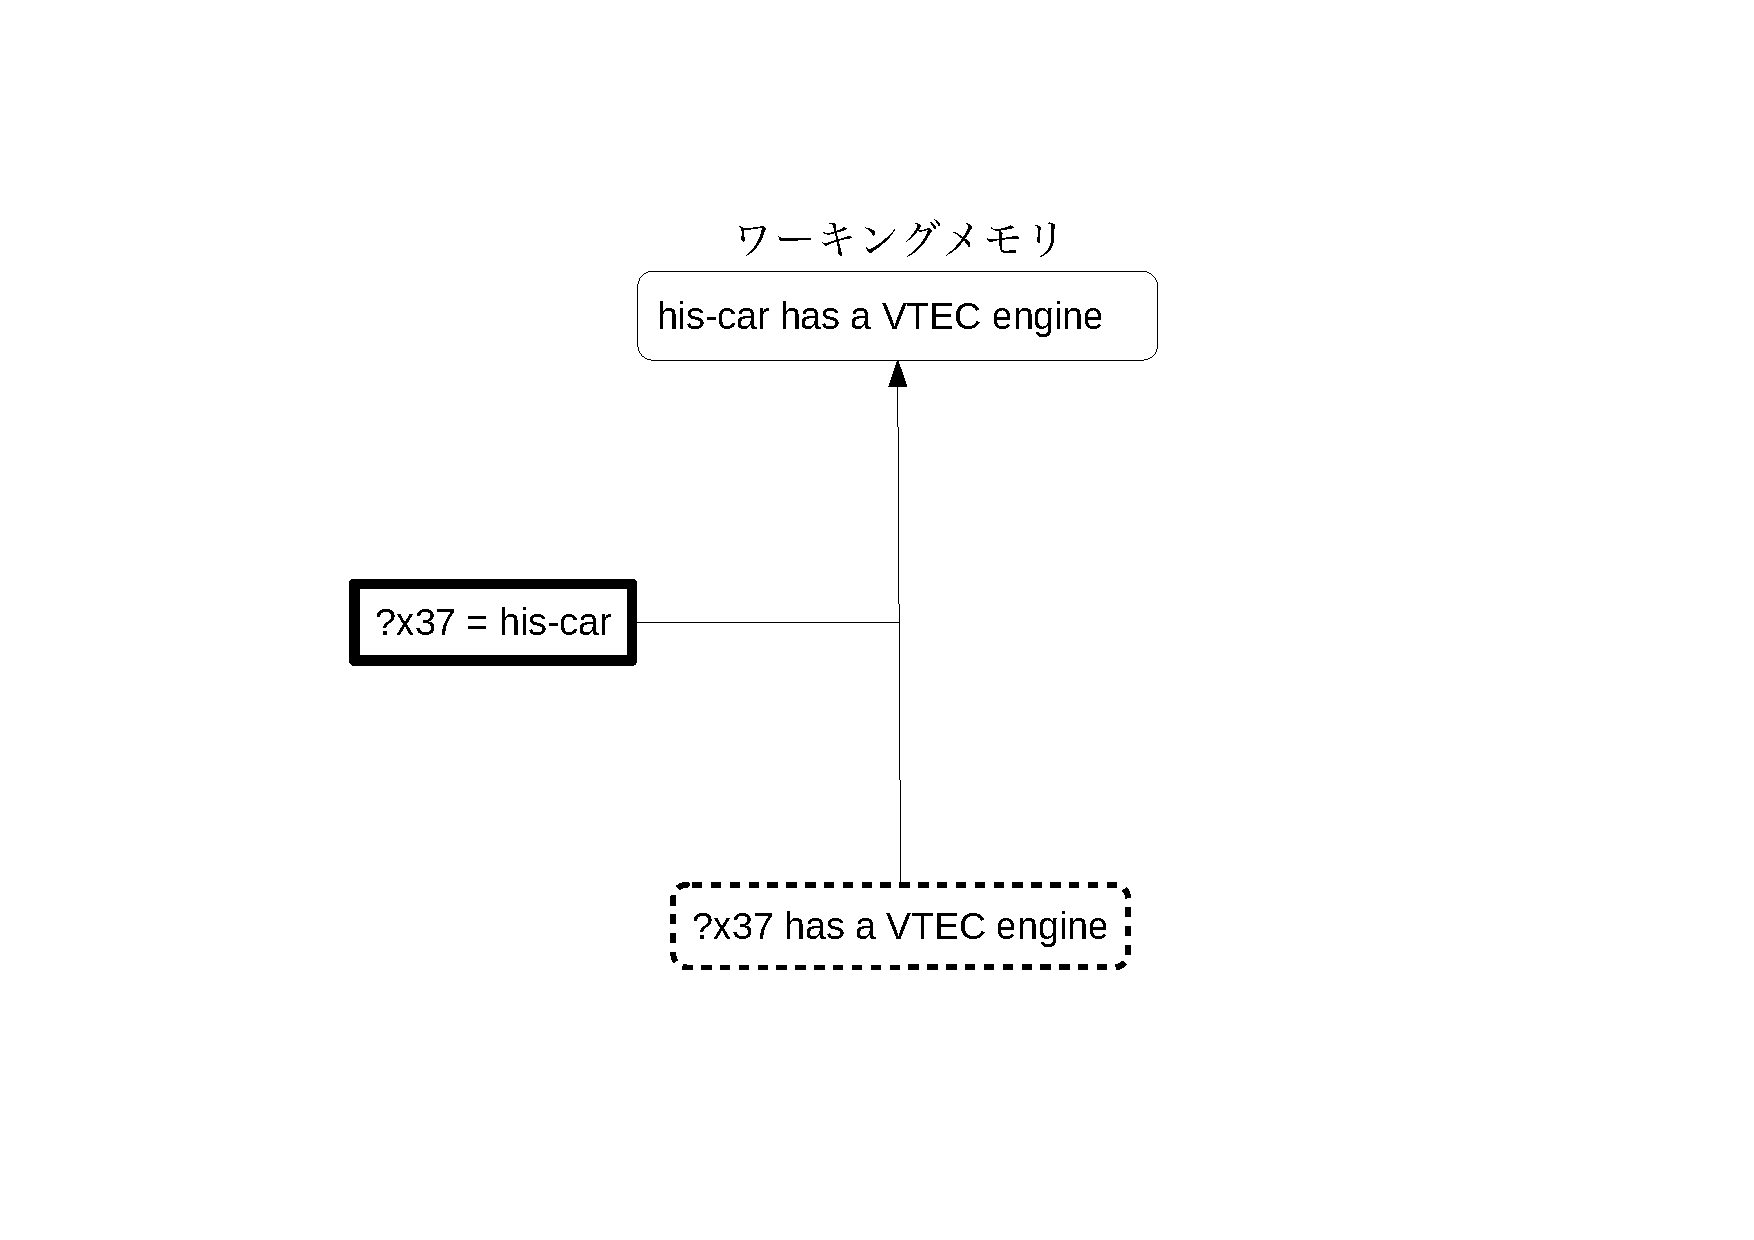
\includegraphics[scale=0.30]{images/backward_chaining_10.pdf}
    \caption{"his-car has a VTEC engine"のチェック}
\end{figure}

\newpage

同様にして,残りの仮説
[his-car is stylish, his-car has several color models, his-car has several seats, his-car is a wagon]
についてもワーキングメモリ内を確認するとそれぞれに該当するアサーションが存在するために仮説が真となることが示される.
以下にこの様子を図15に示す.
\begin{figure}[!hbt]
    \centering
    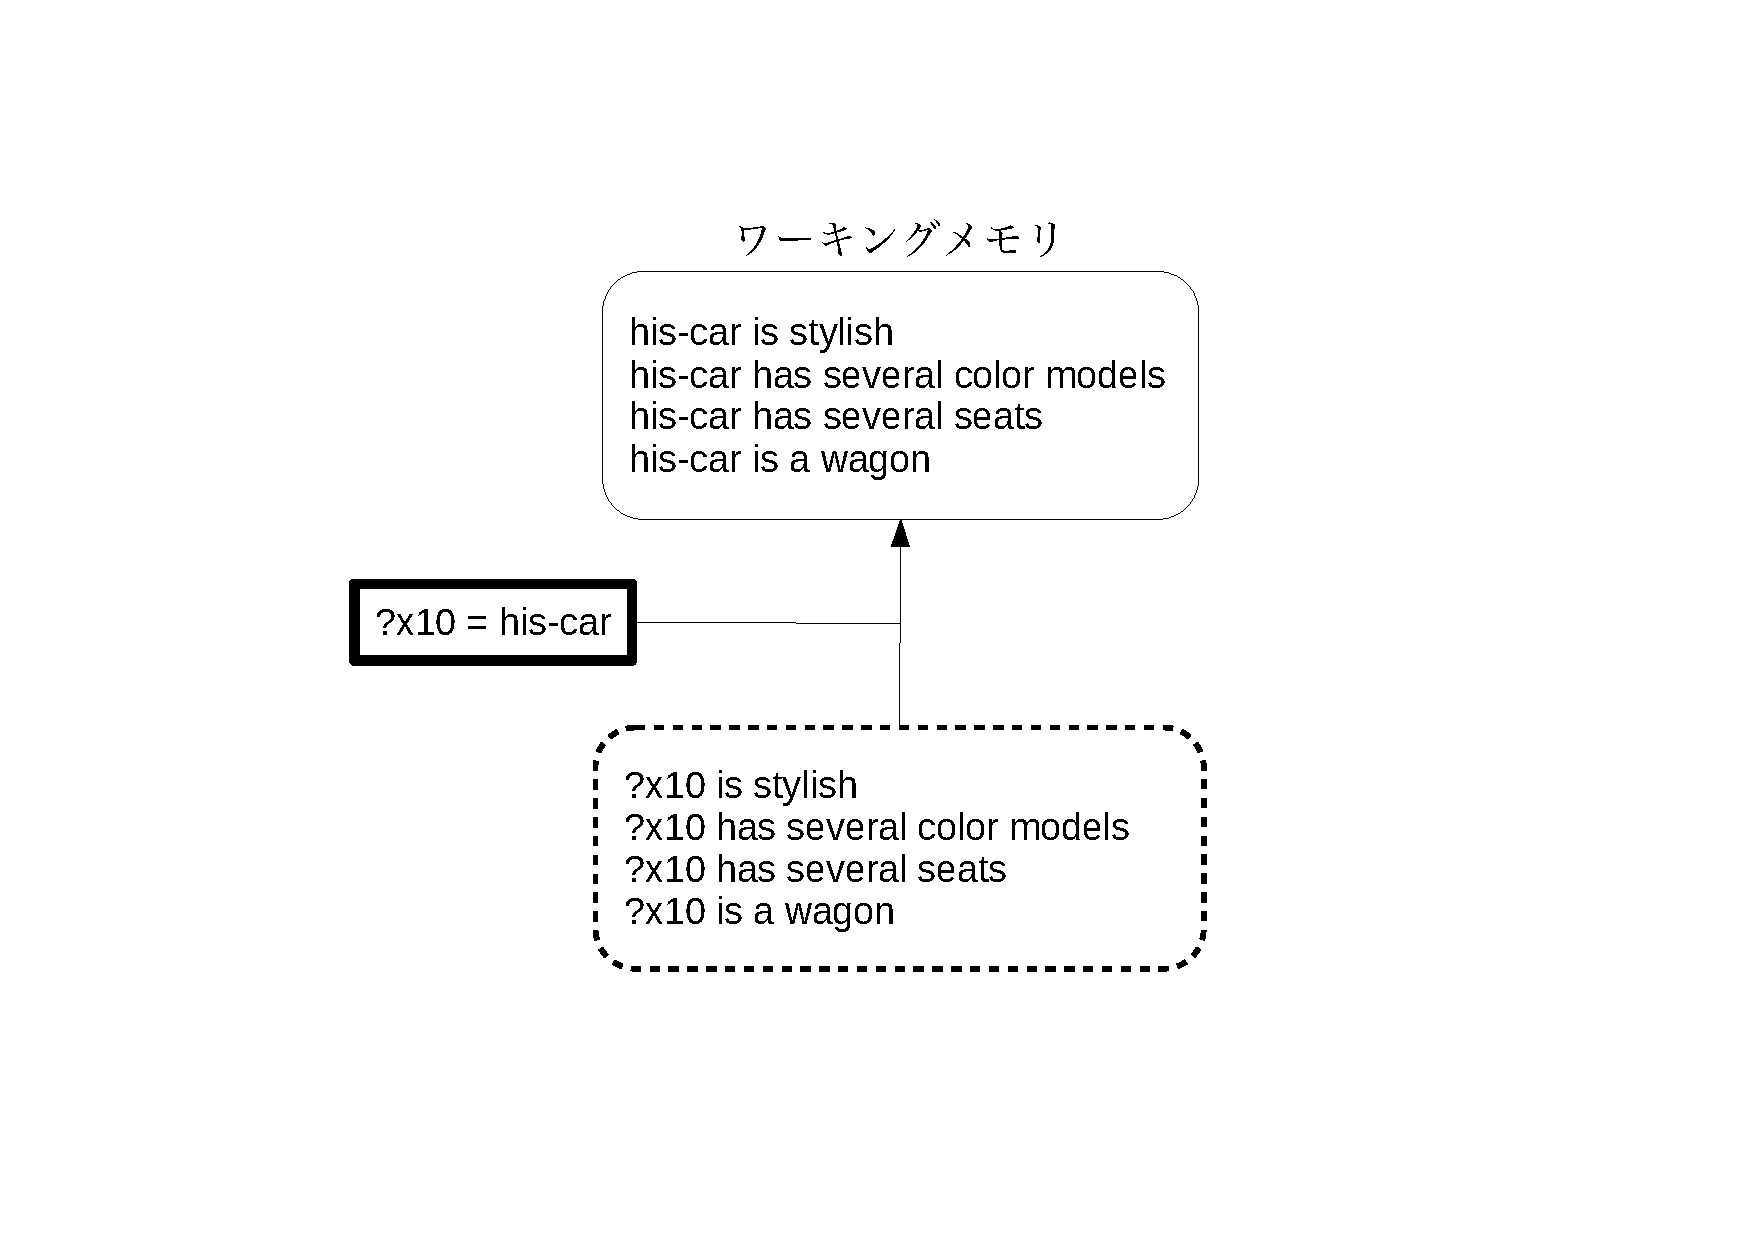
\includegraphics[scale=0.30]{images/backward_chaining_11.pdf}
    \caption{その他の仮説のチェック}
\end{figure}

\newpage

以上によって,?x10=his-carとしてユニフィケーションを行うことで,
CarRule11によって導出された全ての仮説が真となることが示されたので,
元の仮説,"?x is an Accord Wagon"について,?x=his-carが示された.

この後向き推論の成功例の一連の流れを以下の図16に示す.
\begin{figure}[!hbt]
    \centering
    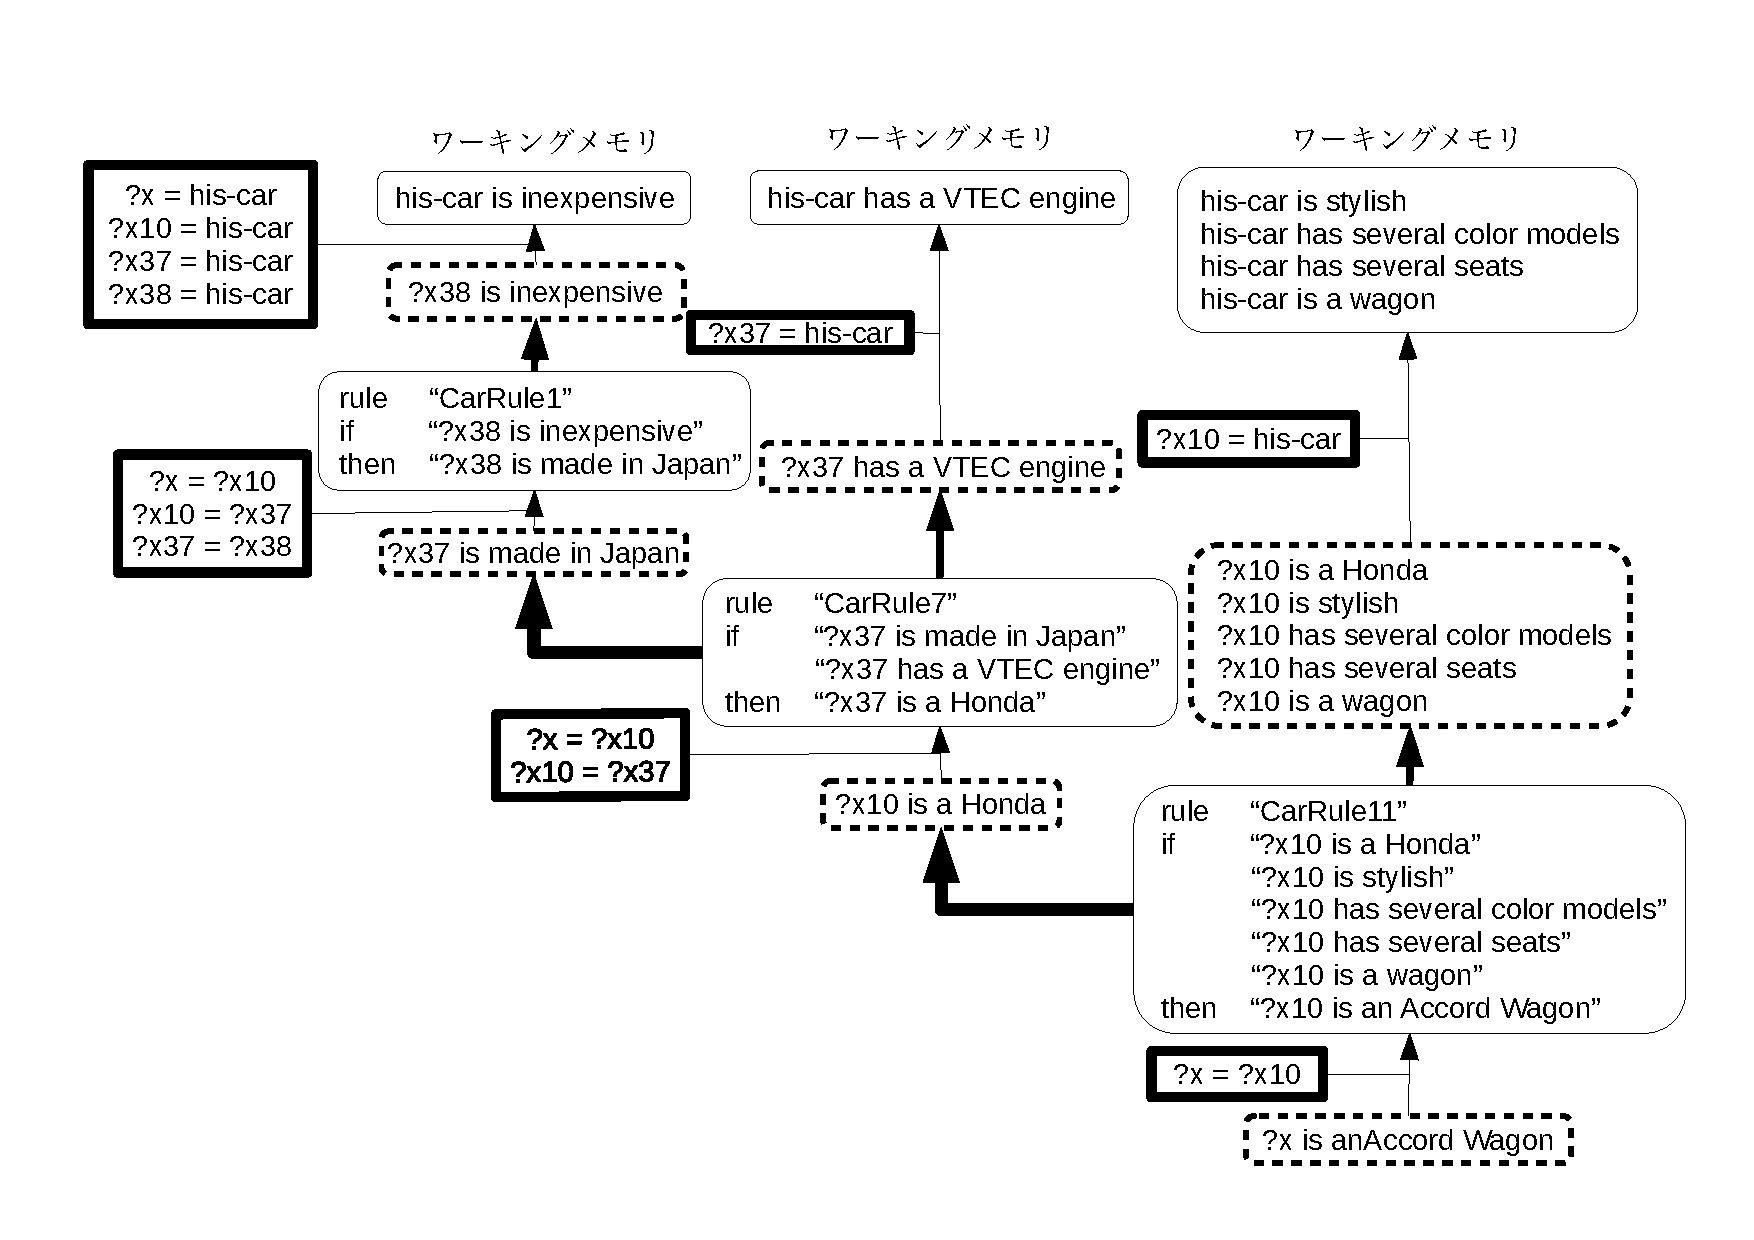
\includegraphics[scale=0.40]{images/backward_chaining_12.pdf}
    \caption{後向き推論の成功}
\end{figure}

\newpage

\subsection{考察}
前向き推論と後向き推論の違いやそれぞれのメリット・デメリットを比較することによって,それぞれの特徴が鮮明になった.
具体的には,前向き推論では網羅的な知識の獲得がなされ,自動的に知識を導き出すといった点での実用がなされるのではないかと考えられる.
対照的に,後向き推論では,その効率性の良さから欲しい知識を応答形式で得ることに特化しているように感じられた. \\
また,前向き推論では,単純な総探索のような形式を取ることによって知識を獲得するので,応答形式を取る際には,あらかじめ下処理として前向き推論を行い,データ検索の際には駆動させない方向で運用すべきであると感じた.
対して,後ろ向き推論では必ず応答形式による利用となることが考えられるため,あらかじめ質問者がどのような知識をどのような形式で質問可能であるかを知っておく必要がある. \\
また,利用されない際には前向き推論による下処理を行い,利用時には後向き推論を利用することにより,さらに効率の良いシステムになるのでは無いかと考えた.
これは,知識量やルールの規模が大きくなるほどに効果を増すのでは無いかと考えられる. \\
知識システムは,知識の量や範囲によって運用の際に制限が大きいのでは無いかと考えられる上に,データ駆動型のシステムとは異なり,全く新しい知識の発見を行うことができない
(入力された知識に依存した範囲でのみの限定的なシステム)であるため,実用的には,こうしたアクセシビリティの面でのブラッシュアップを考える必要があると感じた.


\section{発展課題4-4}
\begin{screen}
    上記4-3で実装したGUIを発展させ,質問応答だけでなく,ルールの編集(追加,削除,変更)などについてもGUIで行えるようにせよ.
\end{screen}
\subsection{手法}
ルールの編集を実装するために,内部処理として二つの段階に処理を分割する.
まず,ルールベース内のルール集合への編集作業を行う.
その次に,変更されたルールベースの内容を,データファイルに上書きする処理を行う.
以上の手順に沿って,実装を行う.

\subsection{実装}
ルールの編集を実装するために,RuleBaseクラス内部に4つのメソッドを新たに追加した. \\

まず,ルールベース内のルールを編集する処理を行うメソッドを作成する.
今回, ルールの編集には,追加,削除,変更の3つが存在するので,それぞれに対応したメソッドを作成する必要がある.
以下に,今回作成した3つのメソッドとその説明を示す.
\begin{description}
    \item[insertRule()] 引数で指定されたルールをルールベースに追加する.
    \item[deleteRule()] 引数で指定されたルールをルールベースから削除する.
    \item[updateRule()] 引数で指定されたルールを変更する.
\end{description}
以上のメソッドによって,ルールベース内部のルール集合に対しての操作がなされる. \\

次に,変更後のルールベースの内容をデータファイルに反映するメソッドwriteFile()を定義する.
このメソッドは,上記の3つのメソッドから共通で利用されるものとする. \\

以上によって,ルールの編集を行う内部実装を行った.

\subsection{実行例}
私(増田)は,ルールの追加・削除・変更を行う実装を担当したため,CUI上での実行結果を示す.
まずは,元のデータファイルを以下に示す.
\begin{lstlisting}[caption=初期のEditRuleTest.data, label=mid]
rule 	"CarRule10"
if 	"?x is a Toyota"
    "?x has several seats"
    "?x is a hybrid car"
then	"?x is a Prius"
\end{lstlisting}
次に,ルールCarRule2を追加する処理を行った際のデータファイルを示す.
\begin{lstlisting}[caption=ルール追加後のEditRuleTest.data, label=mid]
rule	"CarRule10"
if	"?x is a Toyota"
	"?x has several seats"
	"?x is a hybrid car"
then	"?x is a Prius"

rule	"CarRule2"
if	"?x is small"
then	"?x is made in Japan"
\end{lstlisting}
続いて,先ほど追加したルールCarRule2を削除したデータファイルを示す.
\begin{lstlisting}[caption=ルール削除後のEditRuleTest.data, label=mid]
rule	"CarRule10"
if	"?x is a Toyota"
    "?x has several seats"
    "?x is a hybrid car"
then	"?x is a Prius"
\end{lstlisting}
最後に,ルールcarRule10を変更するプログラムを実行した結果を示す.
ただし,二番目の前件を削除する変更を行うとする.
\begin{lstlisting}[caption=ルール変更後のEditRuleTest.data, label=mid]
rule	"CarRule10"
if	"?x is a Toyota"
	"?x has several seats"
then	"?x is a Prius"
\end{lstlisting}

\subsection{考察}
ルールの編集を実装するに当たって2通りの実装方法を考案した.
一つ目の手法は,上述した通り,ルールベース内部のルール集合への編集を行い,操作後のルールベースの内容をデータファイルに上書きする手法である.
二つ目の手法は,データファイルを直接編集することによって,ルールを更新し,再び読み込んでルールベースを構築する手法である.
そこで,データファイルを直接変更することは複雑かつ非効率であるのに対して,
ルールベース内部のルール集合を直接編集する方が容易であると考えたため,前者を選ぶこととした. \\
また,処理を二段階に切り分けることによって,同様の処理をwriteFile()メソッドに統合し,機能の差分をそれぞれ3つのメソッドに任せることで柔軟な構成を作ることができたと考えている.

% 参考文献
\begin{thebibliography}{99}
\bibitem{notty} Javaによる知能プログラミング入門 --著:新谷 虎松 \\
\bibitem{notty} LibreOffice Drawを用いた図版作成 --基礎プログラミング演習I資料(京都産業大学) (2019年11月12日アクセス)\\
\url{http://www.cse.kyoto-su.ac.jp/~oomoto/lecture/program/LibreOffice/draw/index-j.html} 
\bibitem{notty} LaTeXの表を生成できるサイト Tables Generator --muscle\_keisukeの日記 (2019年11月12日アクセス)\\
\url{http://muscle-keisuke.hatenablog.com/entry/2016/07/02/170205} 
\bibitem{notty} LaTeX Tables Generator --Tables Generator (2019年11月12日アクセス)\\
\url{http://www.tablesgenerator.com/latex_tables} \\
\end{thebibliography}

\end{document}